\documentclass[UTF8,a4paper,zihao=-4,fontset=fandol]{ctexart}
% Preamble for Thesis v2 (XeLaTeX + ctexart, minimal clean baseline)
\usepackage{geometry}
\geometry{a4paper, left=2.6cm, right=2.6cm, top=2.8cm, bottom=2.8cm}
\usepackage{amsmath, amssymb, mathtools}
\usepackage{booktabs, longtable, array, tabularx}
\usepackage{graphicx}
\usepackage{float}
\usepackage{siunitx}
\usepackage{xcolor}
\usepackage{hyperref}
\usepackage{cite}

\hypersetup{
  colorlinks=true,
  linkcolor=blue!60!black,
  citecolor=blue!60!black,
  urlcolor=blue!60!black,
  pdftitle={AI辅助下的DRAM存储器单粒子效应评估研究}
}

\graphicspath{{figures/}}

% 显式数据待补标记：严禁把未完成实验或外部缺失数据写成已完成结论
\newcommand{\pendingdata}[1]{%
  \noindent\fcolorbox{orange!70!black}{orange!8}{%
    \parbox{\dimexpr\linewidth-2\fboxsep-2\fboxrule\relax}{%
      \small\textbf{【待补充实测/证据】}\ #1%
    }%
  }\par\vspace{0.4em}%
}

\hypersetup{pdftitle={AI辅助下的DRAM存储器单粒子效应评估研究}}
\title{\heiti\Large AI辅助下的DRAM存储器单粒子效应评估研究\\[0.5em]\large 毕业设计论文（初稿）}
\author{}
\date{\EvidenceDate}

\begin{document}
\maketitle
\begin{abstract}
随着 DRAM 特征尺寸持续微缩，存储节点电容减小、单粒子效应（SEE）敏感度上升，传统依赖束流辐照实验的评估方法成本高、周期长。本文围绕空间高能质子、重离子及大气中子引发的 DRAM 单粒子效应，采用 Geant4 粒子输运与 TCAD 器件仿真联合建模，构建从粒子沉积到读出裕量的可审计数据链路；在此基础上建立数据驱动的单粒子翻转截面与错误率预测模型，开展超参数优化、分组交叉验证与独立性评估，并与仿真/实验结果对比分析关键影响因素。

已有阶段工作表明：在冻结的二维代表模型上，64 个独立粒子事件的 128 条 bit0/1 配对响应可按匹配对照严格分类（5\mV 主阈值下 96 正确、20 判据误读、8 临界、4 数值不确定），基于沉积电荷等特征的岭回归基线在原划分下域内读出裕量退化 MAE 约 0.53--0.55\mV。v4 阶段在厚硅输运与三维源接口上取得阶段性资格证据（212 个初级事件、9 条核非弹性记录见证），r0.6 排批正在推进 P0 资格门与 D0--D3 第一波开发锚点。

本文的贡献边界：模型未作真实器件工艺校准，结果限于原冻结设计与代表模型；截面/错误率需要注量、有效被测比特数等统计分母，目前仅能作条件响应与仿真内验证；导师课题组 DDR5 实验原始数据尚待交接，外部泛化对比为待补章节。全文所有定量结论均可回溯到 run ID、输入/输出哈希与证据索引。
\end{abstract}
\noindent\textbf{关键词：}DRAM；单粒子效应；Geant4；TCAD；数据驱动预测；交叉验证

\tableofcontents
\newpage

% 第1章 研究背景与文献综述
% 证据：tcad-research-training/shared/research-brief.md（导师四项任务与正式题名）；
%       tcad-research-training/shared/literature/mentor-added-20261116.md（L01-L09/J01 拆解）；
%       tcad-research-training/shared/literature/README.md（资料索引与 SHA 清单）；
%       docs/sources/mentor-final-brief.png、mentor-final-title.png（任务与题名截图）；
%       题目_AI辅助下的多特征尺寸存储器单粒子效应评估.md（项目设计大纲提取稿，DOCX SHA256 6ca28c8a…a304）
\section{研究背景与文献综述}

\subsection{研究背景与意义}

动态随机存取存储器（DRAM）以存储电容上的电荷表示信息，访问晶体管导通后存储节点与位线通过电荷共享产生小幅电压差，读出电路据此判断存储状态\cite{keeth2001}。随着特征尺寸持续微缩，存储电容减小、节点电荷减少，单个高能粒子在硅中产生的电子-空穴对经漂移、扩散被节点收集后，就可能改变读出结果，即单粒子效应（SEE）\cite{label1996,baumann2005}。空间环境中的高能质子、重离子以及大气中子是引发 DRAM 单粒子翻转的主要来源。

传统的 SEE 评估高度依赖加速器束流辐照实验：器件筛选、注量累积、错误日志解析都需要机时和样品，成本高、周期长，且难以覆盖全部工艺与粒子工况。因此，将 Geant4 粒子输运仿真与 TCAD 器件仿真联合，并结合数据驱动的预测模型，用有限的实验与仿真数据挖掘多维参数规律、预测翻转截面与错误率，成为降低辐照试验依赖的一条技术路线。这正是导师下发任务的核心动机：调研评估方法与 AI 应用现状，构建 Geant4/TCAD 模型与数据集，建立并训练预测模型，最后与仿真/实验结果对比评价精度与泛化能力\cite{mentortask}。

\subsection{DRAM 单粒子效应评估的研究现状}

\subsubsection{Geant4 与 TCAD 联合仿真}
Geant4 适于描述载能粒子在材料中的输运与能量沉积，TCAD 适于描述器件内部的电荷收集与瞬态电学响应，二者的耦合是 SEE 仿真的主流方法。陈善强等将 TCAD 与 Geant4 用于 SRAM 单粒子效应评估\cite{chen2011}；罗捷等用 Geant4 模拟 Bi、Xe、Kr 的径向沉积并输入 Sentaurus 分析电荷收集，指出 LET 相同也不能保证径向分布相同，粒子种类、能量、位置、时间与通量都应保留在数据链中，其每比特截面定义为 $\sigma_{bit}=N_{bit\ errors}/(\Phi \times N_{tested\ bits})$，分母包含粒子注量与被测比特数\cite{luo2018}。这些工作为本文的 Geant4→TCAD 参数传递与统计分母口径提供了方法依据，但其 SRAM/NMOS 对象与通量阈值不直接照搬到 DRAM。

\subsubsection{器件级建模与校准}
Ryu 等对 14 nm saddle-fin DRAM 开展重离子 TCAD 仿真，给出了结构与 I--V 校准流程，并指出直接收集与邻近节点共享对温度的响应不同，不能用一句"温度越低越抗辐射"概括\cite{ryu2025}；Aditya 等用 14 nm SOI FinFET eDRAM 的 mixed-mode TCAD 分析方向、位置与读出阈值，其报告的临界 LET 依赖特定的读出阈值与电路设置，不是通用值\cite{aditya2018}。这些文献说明：器件模型必须有明确的结构、校准与适用边界，电压下降、共享电荷与最终读错需要分开表述。

\subsubsection{实验表征与错误分类}
Memon 等在 20--58 MeV 质子束下对 COTS LPDDR2/LPDDR4 开展应力测试，按访问图样分组报告计数、注量、截面与不确定度，并强调日志不可解析不等于零错误、SoC 制程与 DRAM 制程不能混用\cite{memon2025}。Jin 等指出 DRAM 的软错误率失效包含阵列位翻转与外围锁存器翻转导致的 SEFI 两类机制，加固比例的分母和层级不同，不能直接当绝对截面\cite{jin2026}。Baumann 的综述区分了 SEU/MBU/SEFI 与节点电荷到系统可见失效的关系\cite{baumann2005}。这些工作为本文的标签统一（瞬态响应、位翻转、SEFI、保持退化分开）与统计分母规范提供了依据。

\subsection{AI 在辐射效应评估中的应用现状}

机器学习已被用于电路级单粒子瞬态的回归建模\cite{xu2021}；Ryder 等比较重离子、聚焦 X 射线与脉冲激光诱导的响应，指出生成电荷总量相近不保证器件瞬态一致，空间分布仍影响响应\cite{ryder2021}。纪志罡的讲义从 DRAM 可靠性的跨层优化视角，讨论了"物理量/波形 → 参数 → 电路指标"的分层代理、图神经网络/迁移学习/PINN 等方法，并强调训练特征应有物理来源、经验拟合好不代表外推可靠\cite{ji2026}。共同趋势是：先建立可解释的简单基线，再比较非线性代理与物理约束模型，并按器件或独立事件分组划分训练/测试，同时报告精度与计算成本。

\subsection{现有不足与本文切入点}

综合上述文献与导师新增资料包，现有工作在以下方面仍有不足：第一，仿真数据集的标签与分母不统一，瞬态响应、判据误读、持久翻转、SEFI 容易混为一谈；第二，Geant4 到 TCAD 的传递与数值验证缺乏可审计的证据链，复跑容易被误当作独立样本；第三，AI 预测多以拟合精度为主，缺少物理约束消融与独立留出的泛化验证；第四，截面/错误率常缺少注量、有效容量与观测时间等分母，难以与实验对照。

本文的切入点是：以可追溯的 Geant4/TCAD 联合仿真链路为基础，统一指标与标签口径，构建带 run ID 与哈希的合格数据集；在此基础上建立数据驱动预测模型并开展超参优化与分组交叉验证，与仿真结果及（待交接的）实验数据对比，分析关键影响因素。

\subsection{研究内容与技术路线}

对应导师任务的四项工作，本文安排为七章：第 2 章介绍 Geant4/TCAD 联合建模与数据链路；第 3 章介绍数据集构建与质量门槛；第 4 章介绍 AI 预测模型、超参优化与交叉验证；第 5 章报告实验结果；第 6 章讨论误差、失败案例与适用边界；第 7 章总结结论与后续工作。技术路线为"已有 DRAM 模型与证据 → 单粒子电学响应和有效读出 → 有统计分母的数据集 → AI 预测与独立验证"。

\subsection{论文组织结构}

第 1 章为背景与文献综述；第 2--4 章为方法（建模、数据集、预测模型）；第 5--6 章为结果与讨论；第 7 章为结论。每章的素材来源、哈希与适用边界统一记录在 \texttt{materials/素材索引.md}，正文定量结论均可回溯。

% 第2章 Geant4/TCAD 联合建模与数据链路
% 证据：tcad-research-training/experiments/plan.md（v3 冻结设计与授权记录）；
%       tcad-research-training/shared/metrics-and-labels.md（指标/标签口径，v3 已冻结实现）；
%       tcad-research-training/experiments/dram-see-v4/device-basis.md（器件参数来源与待校准项）；
%       tcad-research-training/experiments/dram-see-v4/README.md（v4 阶段成果：212 初级事件、9 核非弹性见证、三维源账本）；
%       tcad-research-training/experiments/dram-see-v3/r50-main/final-delivery-r4.md（64 事件/128 响应冻结交付）；
%       output/server-benchmark-20261115/REPORT.md（云端平台与基准）；
%       tcad-research-training/plans/dram-se-ddr5-lpddr5/P0-CLOSEOUT-AND-D0-D3-FIRST-WAVE-PREP-r06-20261120.md（r0.6 当前排批）
\section{Geant4/TCAD 联合建模与数据链路}

\subsection{器件模型与参数来源}

本文采用 1T1C（一管一容）DRAM 存储单元作为代表模型：访问晶体管加存储电容，保留电荷共享与器件输运的基本物理，暂不模拟完整阵列、真实感放与恢复电路。历史探索在二维 0.18/0.25/0.35/0.45\um 等效单元上完成（v3 冻结设计），v4 阶段转向以 BCAT 为代表的三维结构，并登记了 g70/g80/g90 埋栅顶深等几何变量（注意：这些数值指埋栅顶深，不是商业工艺节点）。

器件参数来源分两类：一是公开文献，如 Shin 等给出的 90 nm DRAM 栅长约 95 nm、栅堆叠 poly-Si 80 nm / WSi$_x$ 100 nm / Si$_3$N$_4$ 180 nm 等结构信息\cite{shin2003}；二是导师提供的 LPDDR5 规格资料（JESD209-5 与 Micron LPDDR5 datasheet），用于命令、刷新与电气边界，但不能由外部封装规格反推内部掺杂或栅长\cite{jesd209-5,micronlpddr5}。当前模型**未作真实器件 I--V/保持/读出校准**，有效沟道宽度、结深、掺杂剖面、Cstore 等参数仍列在待校准清单中；仅调到一条曲线吻合不能反推真实工艺参数。因此本文所有器件级结论均限于"未校准代表模型"的适用范围。

\subsection{Geant4 粒子输运模型}

输运端记录粒子种类、能量、入射位置与方向、事件数、随机种子与物理列表版本。v3 冻结设计采用固定 5 MeV、两种入射角度与固定入射位置的 64 个独立事件；v4 阶段在独立三维厚硅体中完成了 212 个初级质子事件的记录检查（保留 66 条轨迹、1724 个步骤），并取得 9 条核非弹性记录作为核机制见证，同时保留了两次零沉积射偏事件的失败记录；三个三维源账本已闭合。r0.6 排批当前以 P0 资格门（数值重复性、PMI 日志链、时序保持窗、源积分）和 D0--D3 四个开发锚点（nominal / short-channel / narrow-fin / …）为第一波正式范围。

输运输出的审计包括：事件/轨迹/parent 关系、材料、时间、零沉积与核过程记录，以及源积分的相对误差硬核验（要求有限且 $<10^{-9}$）。同种子的前后复测不增加独立事件数。

\subsection{Geant4 到 TCAD 的参数传递}

传递链路为"粒子输运 → 能量沉积 → 电子-空穴对 → 等效径迹源 → TCAD 激励"。字段定义包括单位换算、坐标变换、区域筛选、沉积量到源项的离散化与时间分配，二维采用等效源近似，三维保留空间投影。接口合同要求每条源记录绑定几何、物理列表/数据版本、种子与输入身份；完全匹配的 A0 对照或输运可复用，模型/时序/网格不同则不能直接借用。v4 阶段 A0/A1/A4 三个 TCAD 接口算例已通过，细网格 A0/A1 的全部 205 帧源测量与匹配对照网格比较通过，粗网格空间失败保留未隐瞒。

\subsection{单粒子响应指标与判据}

令 $b\in\{0,1\}$ 为存储位值，signal 为粒子响应，control 为同初态无粒子对照，neutral 为独立中性参考。v3 冻结的连续量定义为：
\begin{itemize}
  \item $\Delta Q_{\fC} = C_{store} \times [V_{sn}^{signal}(2.8\ns) - V_{sn}^{control}(2.8\ns)] \times 10^{15}$（有符号，不取绝对值代替）；
  \item $D_{\mV} = [V_{BL}^{signal}(4\ns) - V_{BL}^{neutral}(4\ns)] \times 10^{3}$；
  \item $M_{\mV} = (2b-1) \times D_{\mV}$；$\Delta M_{\mV} = M_{control} - M_{signal}$，正值为裕量损失；
  \item 读窗 3.8--4\ns，采样分段线性插值；4\ns 单点分类与整个读窗稳定性分开报告。
\end{itemize}

分类标签：$M>\varepsilon$ 为 correct，$M<-\varepsilon$ 为判据误读（criterion\_error，不直接等同已证持久位翻转），$-\varepsilon\le M\le \varepsilon$ 为 critical，数值证据不足为 numerically\_uncertain，求解失败为 failed。v3 主阈值 $\varepsilon=5\mV$，敏感性阈值 2.5/10\mV。每物理条件每 bit 的计划独立事件 $N=4$；同事件的 bit0/1 配对、验证角色、重试均不增加独立事件。持久翻转与 SEFI 需要独立的持续性/功能判据，现有裕量指标不能单独证明。

\subsection{数值验证与失败记录}

数值质量控制采用预登记细化：半时间步与 0.7 网格各自使用自己的事件、对照与中性参考，读出差异与 $\Delta Q$ 差异均在 0.5\mV / 0.01\fC 容差内，三阈值分类保持一致；该结论仅支持预登记点，不代替后续边界检查。失败案例原样保留：例如 v3 训练中固定种子事件在 3\ns 预充偏差 13.297\uV 超过 10\uV 门槛，工程求解成功但科学审计失败，标记 FAILED 并暂停依赖任务，不替换事件或放宽阈值。匹配中性参考的 8/8 无粒子一致性已通过。这些"通过+失败"并存的记录是本文可复现性论述的核心证据。

\subsection{计算平台与运行控制}

仿真平台为个人笔记本加实验室服务器（12 核/32\,GB Rocky9）上的 CentOS 7.9 虚拟机（分配 9 核/28\,GiB），TCAD 只用共享池中的既有配置，Geant4 沿已验证 profile 轮换；云端基准记录了迁移、Geant4 更新前后检查与同条件性能对比，2 并发×4 核为拟实测配置，短测试不外推整月吞吐。运行控制为唯一串行调度者、输入冻结、锁与收集租约沿用原共享池，每次运行保留 run ID、输入 SHA256、种子、退出码、日志哈希与全程资源采样（详见 \texttt{materials/证据收集清单.md}）。

% 第3章 数据集构建与质量门槛（占位，待合格 v4/r0.6 数据导出后填充）
% 素材：tcad-research-training/shared/data-dictionary.md（34 字段合同草案）；
%       experiments/dram-see-v3/r50-main/data/delivery-r4/20261012T0033Z-full/responses.csv（128 响应样例）；
%       experiments/dram-see-v4/source-ledger/（三维源账本）；
%       plans/dram-se-ddr5-lpddr5/matrix.yaml、month-one-cases-r06.json（r0.6 工况矩阵）
% 缺口：G03 合格 v4 响应（匹配 A0、实际源时钟/积分、完整波形、端口电荷）；G04 统计分母
\section{数据集构建与质量门槛}

\textbf{待补章节。} 本章计划覆盖：样本单元（事件+bit+模型+状态+run+哈希）、字段合同、质量门槛（匹配对照、KCL、源积分）、缺失/失败处理与统计分母。已有 v3 冻结数据集（64 独立事件/128 配对响应，快照 20261012T0033Z-full，64/64 哈希核验通过）可作为方法样例，但不与 v4 拼成同质训练集。

% 第4章 AI 预测模型、超参优化与交叉验证（占位，待 A02/A03 完成后填充）
% 素材：tcad-research-training/predictor/README.md（predict-r / predict-f 合同）；
%       experiments/dram-see-v3/r50-main/data/delivery-r4/20261012T0033Z-full/prediction-scores.csv（4 岭回归基线评分，域内 ΔM MAE≈0.53–0.55 mV）；
%       shared/metrics-and-labels.md §5（泄漏控制：同事件/配对 bit/细化归同一组，旧留出再调参不算盲测）；
%       r0.6 决定：R→A→F 残差模型，比较纯机理/浅层树/纯 MLP/RC+残差/RC+残差+KCL
% 缺口：A02 物理约束消融、A03 分组 CV 与冻结盲测
\section{AI 预测模型、超参数优化与交叉验证}

\textbf{待补章节。} 本章计划覆盖：特征合同与泄漏控制、基线（均值/岭回归）与候选模型、开发集内超参选择、按独立事件分组的交叉验证、冻结后独立留出评分、物理一致性（守恒残差）与预测精度的分别报告。历史 v3 岭回归只作为方法基线，不冒充新模型盲测。

% 第5章 实验结果
% 图均为 v3 冻结设计（快照 20261012T0033Z-full）下真实数据生成，哈希核验见
%   tcad-research-training/shared/evidence/reuse-audit-20261116.json 与 materials/图表引用清单.md
% 红线：失败与未决必须出现；配对≠独立事件；不把波形叫实测截面；新 r0.6 结果合格后按 5.7 节补入
\section{实验结果}

本章结果均来自 v3 冻结设计（64 个独立事件 / 128 条 bit0/1 配对响应，数据版本 20261012T0033Z-full），在未校准二维代表模型、固定 5\,MeV 粒子、两种角度与固定入射位置的范围内解释；r0.6 新结果合格后补入 5.7 节。

\subsection{初态与无粒子基线}

图\ref{fig:initial-state} 展示写入后的初态检查，是全部匹配对照的共同起点。8/8 无粒子物理/离线参考一致性已通过，各侧 4\ns 电压差绝对值最大约 $6\times10^{-15}\V$，三阈值分类一致。

\begin{figure}[htbp]
\centering
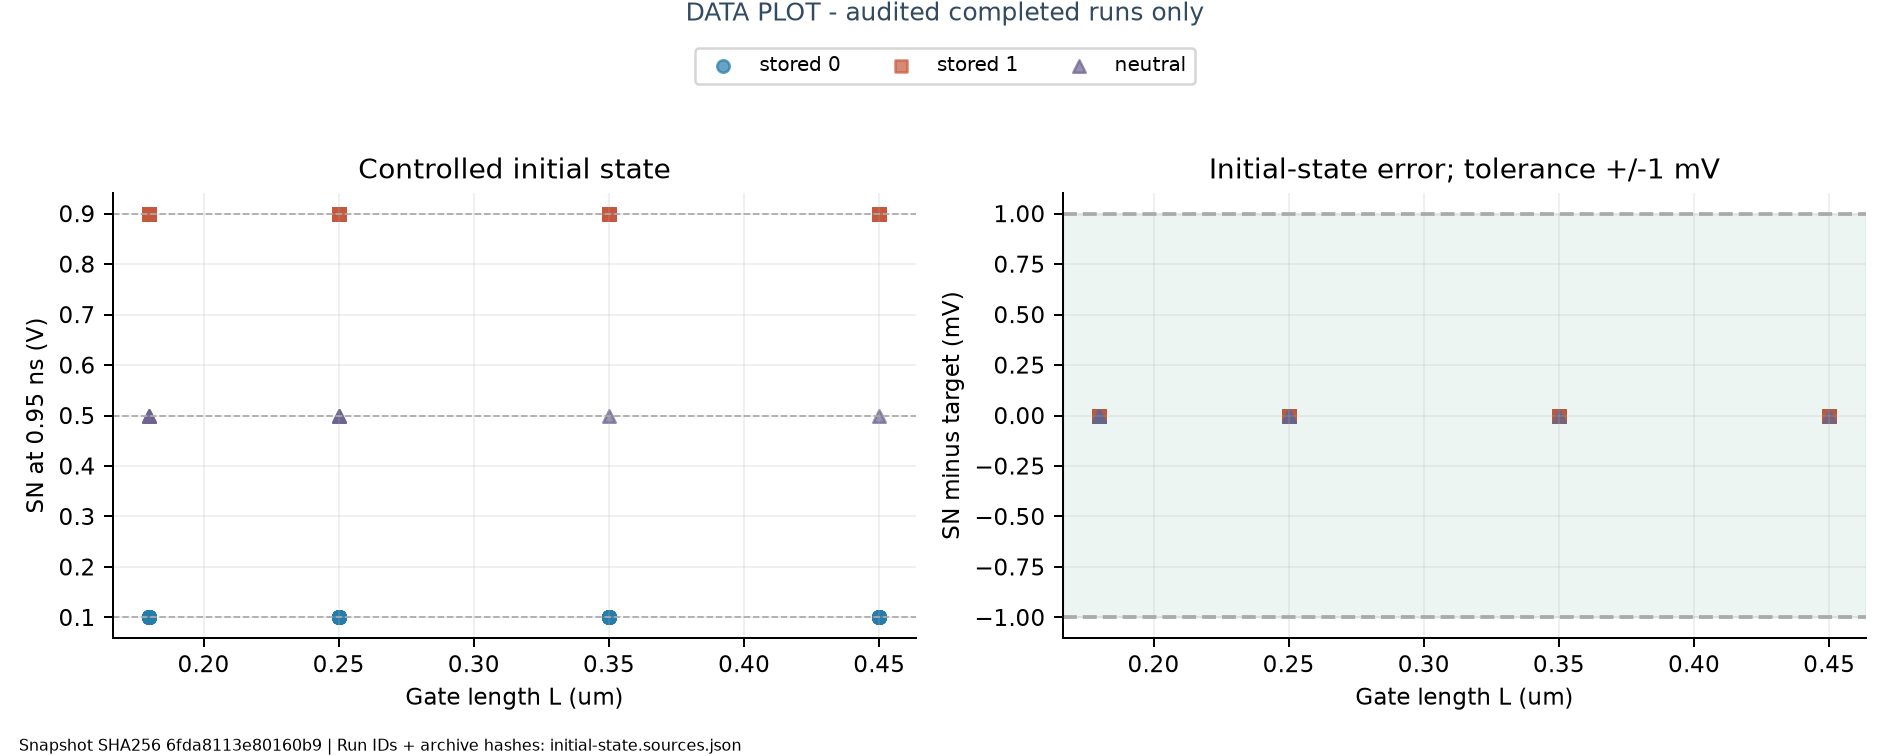
\includegraphics[width=0.8\textwidth]{figures/initial-state.png}
\caption{v3冻结设计下的写入初态检查。数据版本：20261012T0033Z-full；原始 run 与输入/输出哈希见共享证据索引。结果用于未校准代表模型的方法验证；v3 原结构与原时序，不代表真实 DDR5 校准。}
\label{fig:initial-state}
\end{figure}

\subsection{单粒子读出响应与多尺寸比较}

图\ref{fig:readout-l018}--\ref{fig:readout-l045} 给出四种栅长下相同事件/bit/对照的波形与读出裕量。固定 5\,MeV、固定入射位置与原二维代表模型；判据误读不等于持久位翻转。

\begin{figure}[htbp]
\centering
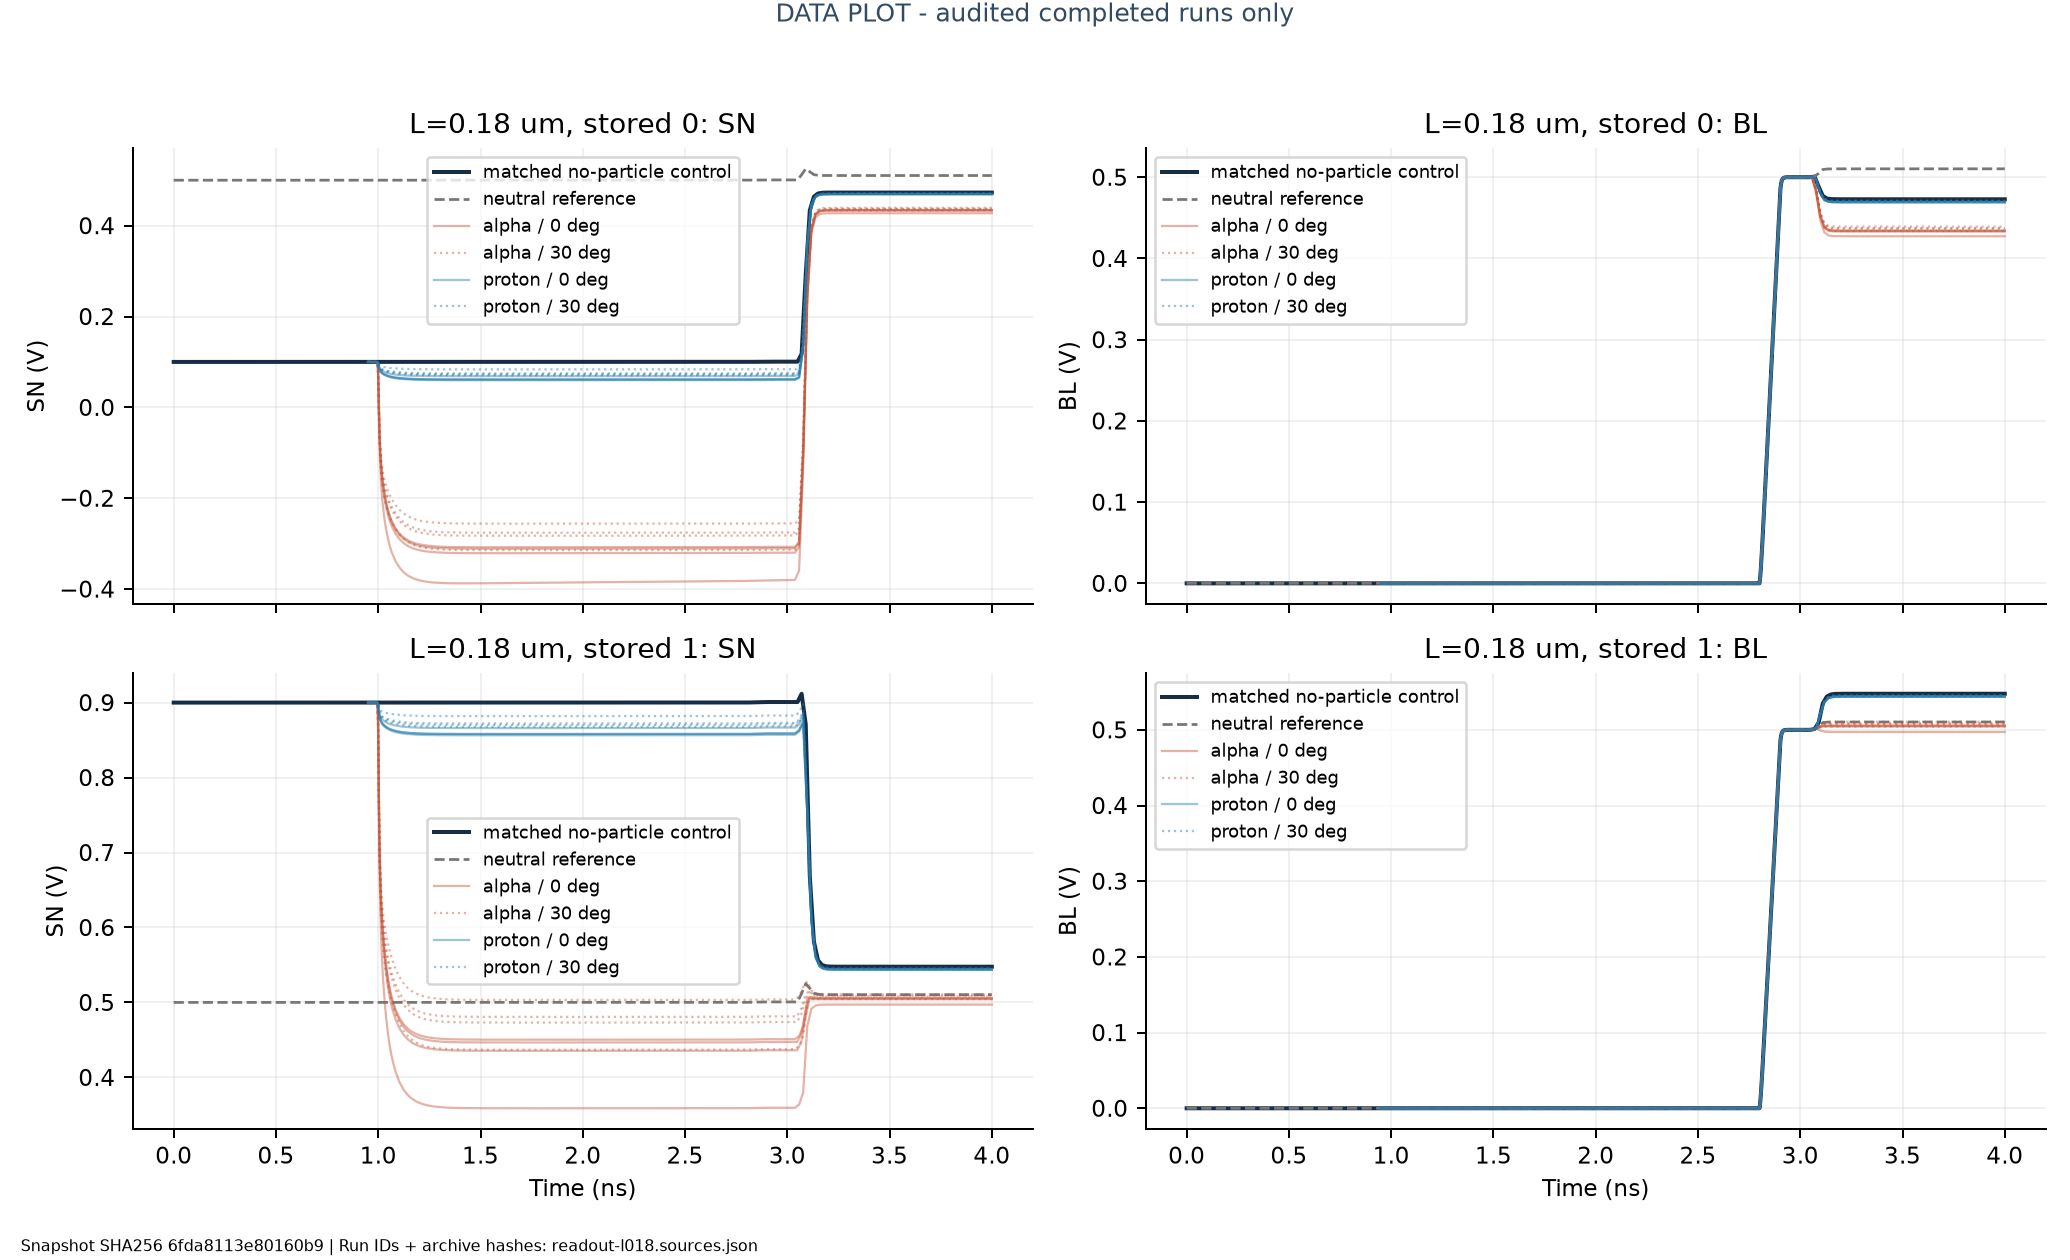
\includegraphics[width=0.48\textwidth]{figures/readout-l018.png}
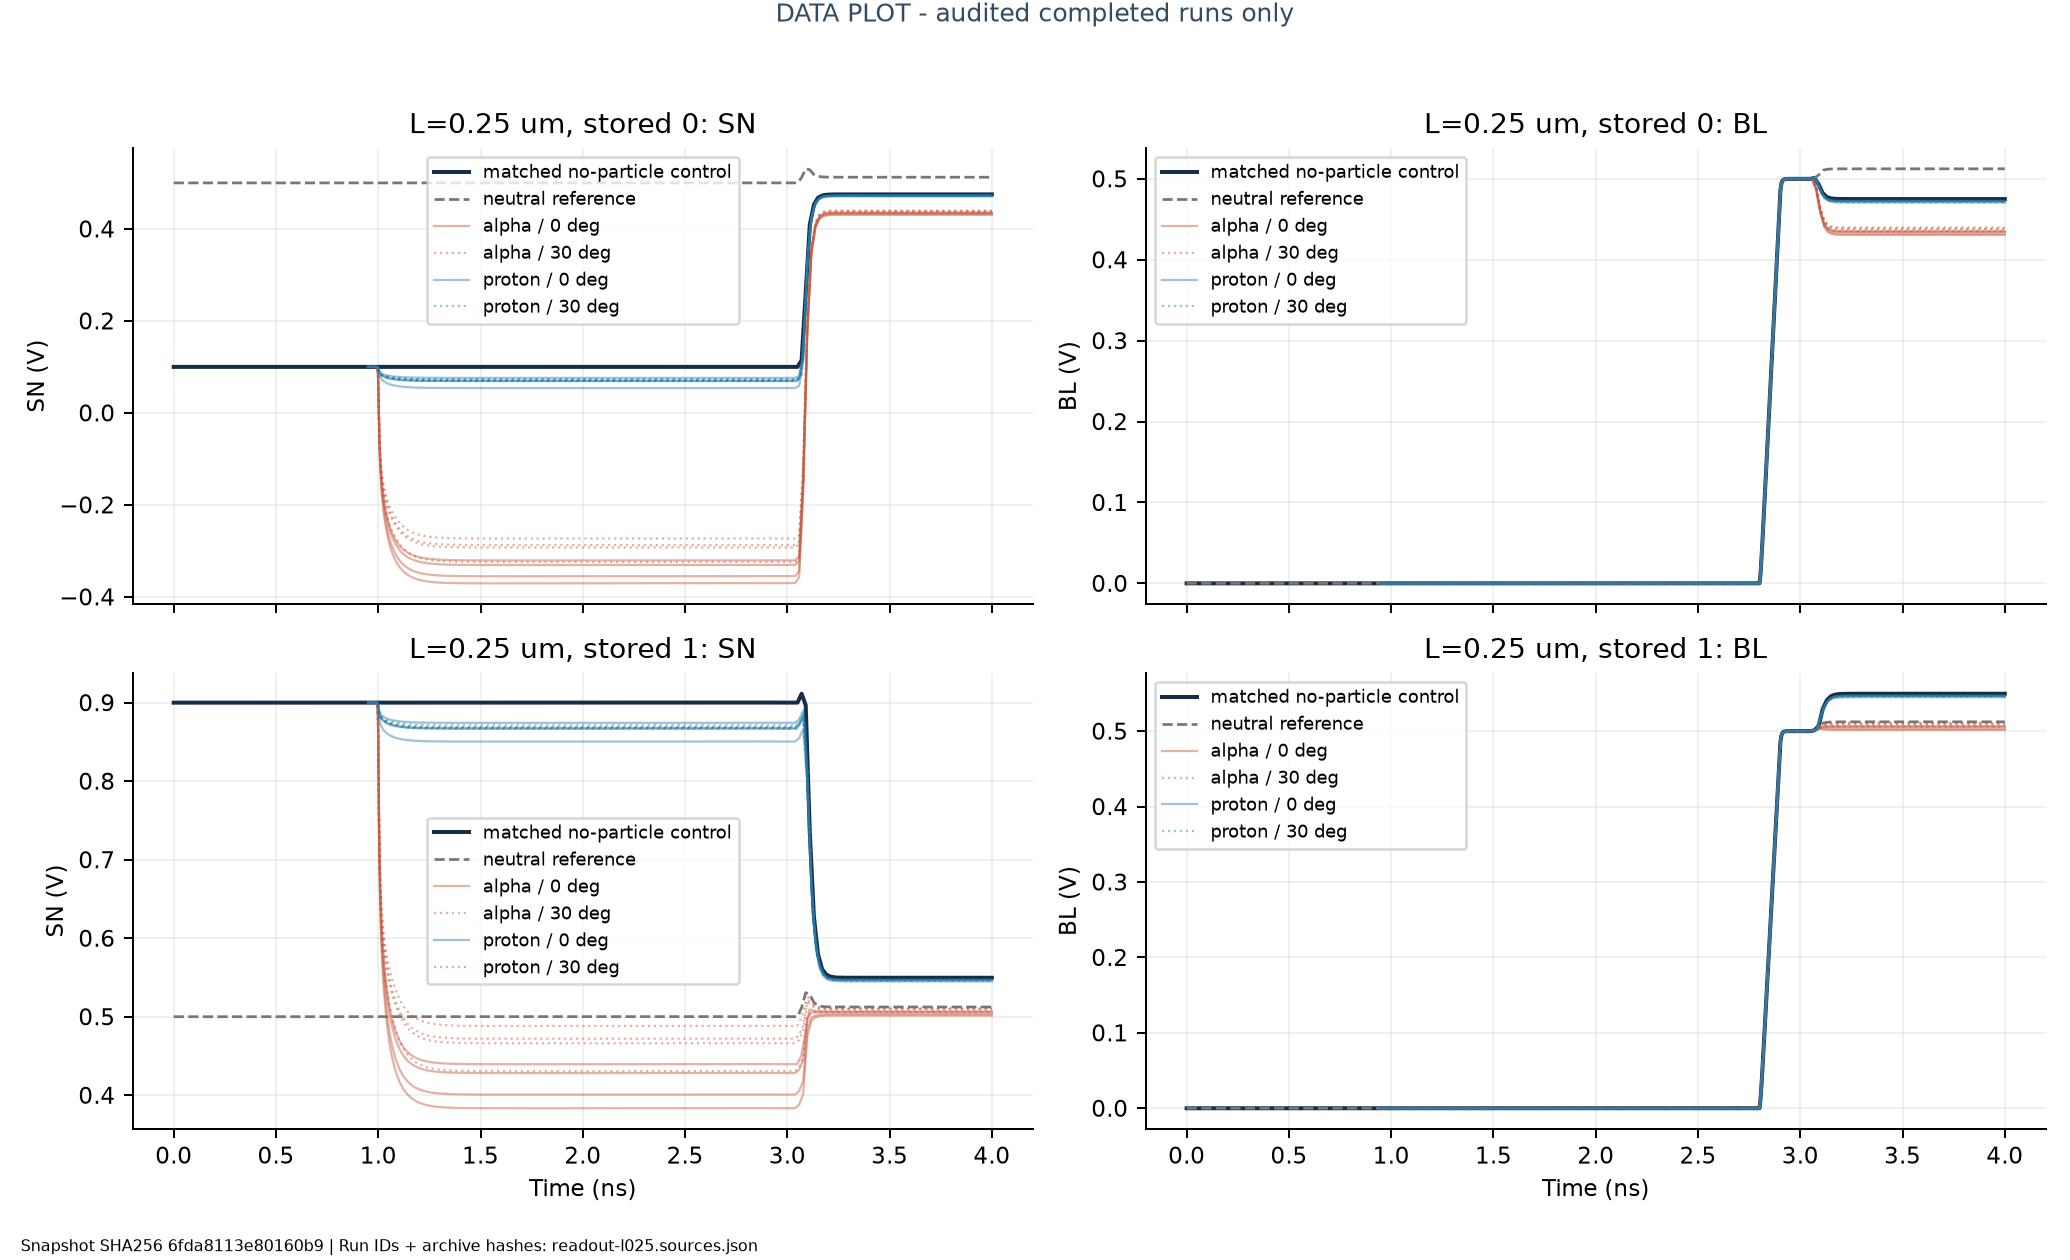
\includegraphics[width=0.48\textwidth]{figures/readout-l025.png}
\caption{v3冻结设计下 0.18/0.25\um 读出响应波形。数据版本：20261012T0033Z-full；固定 5\,MeV、固定位置、原二维代表模型。}
\label{fig:readout-l018}
\end{figure}
\begin{figure}[htbp]
\centering
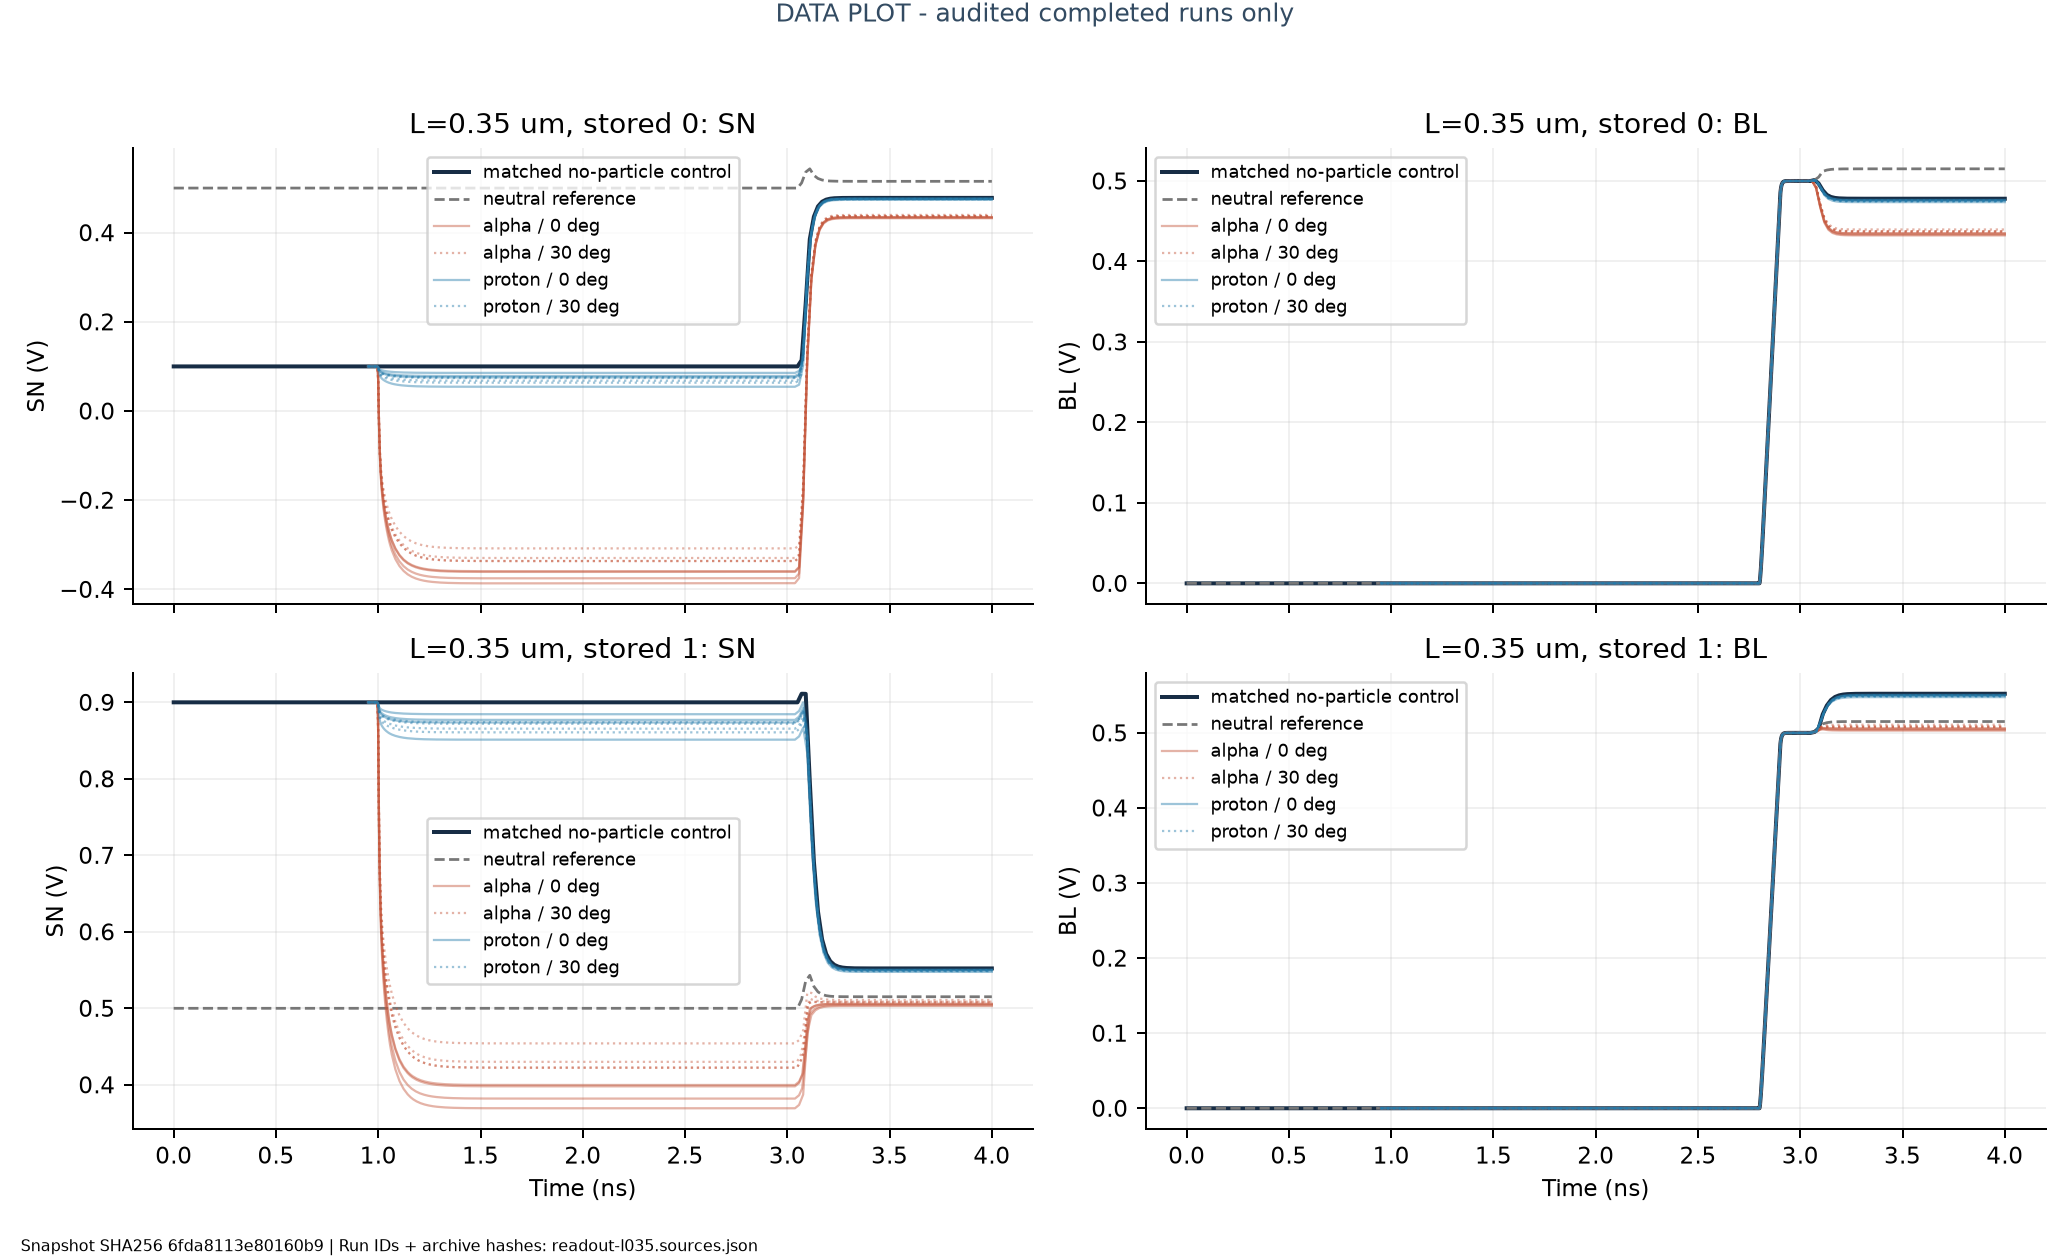
\includegraphics[width=0.48\textwidth]{figures/readout-l035.png}
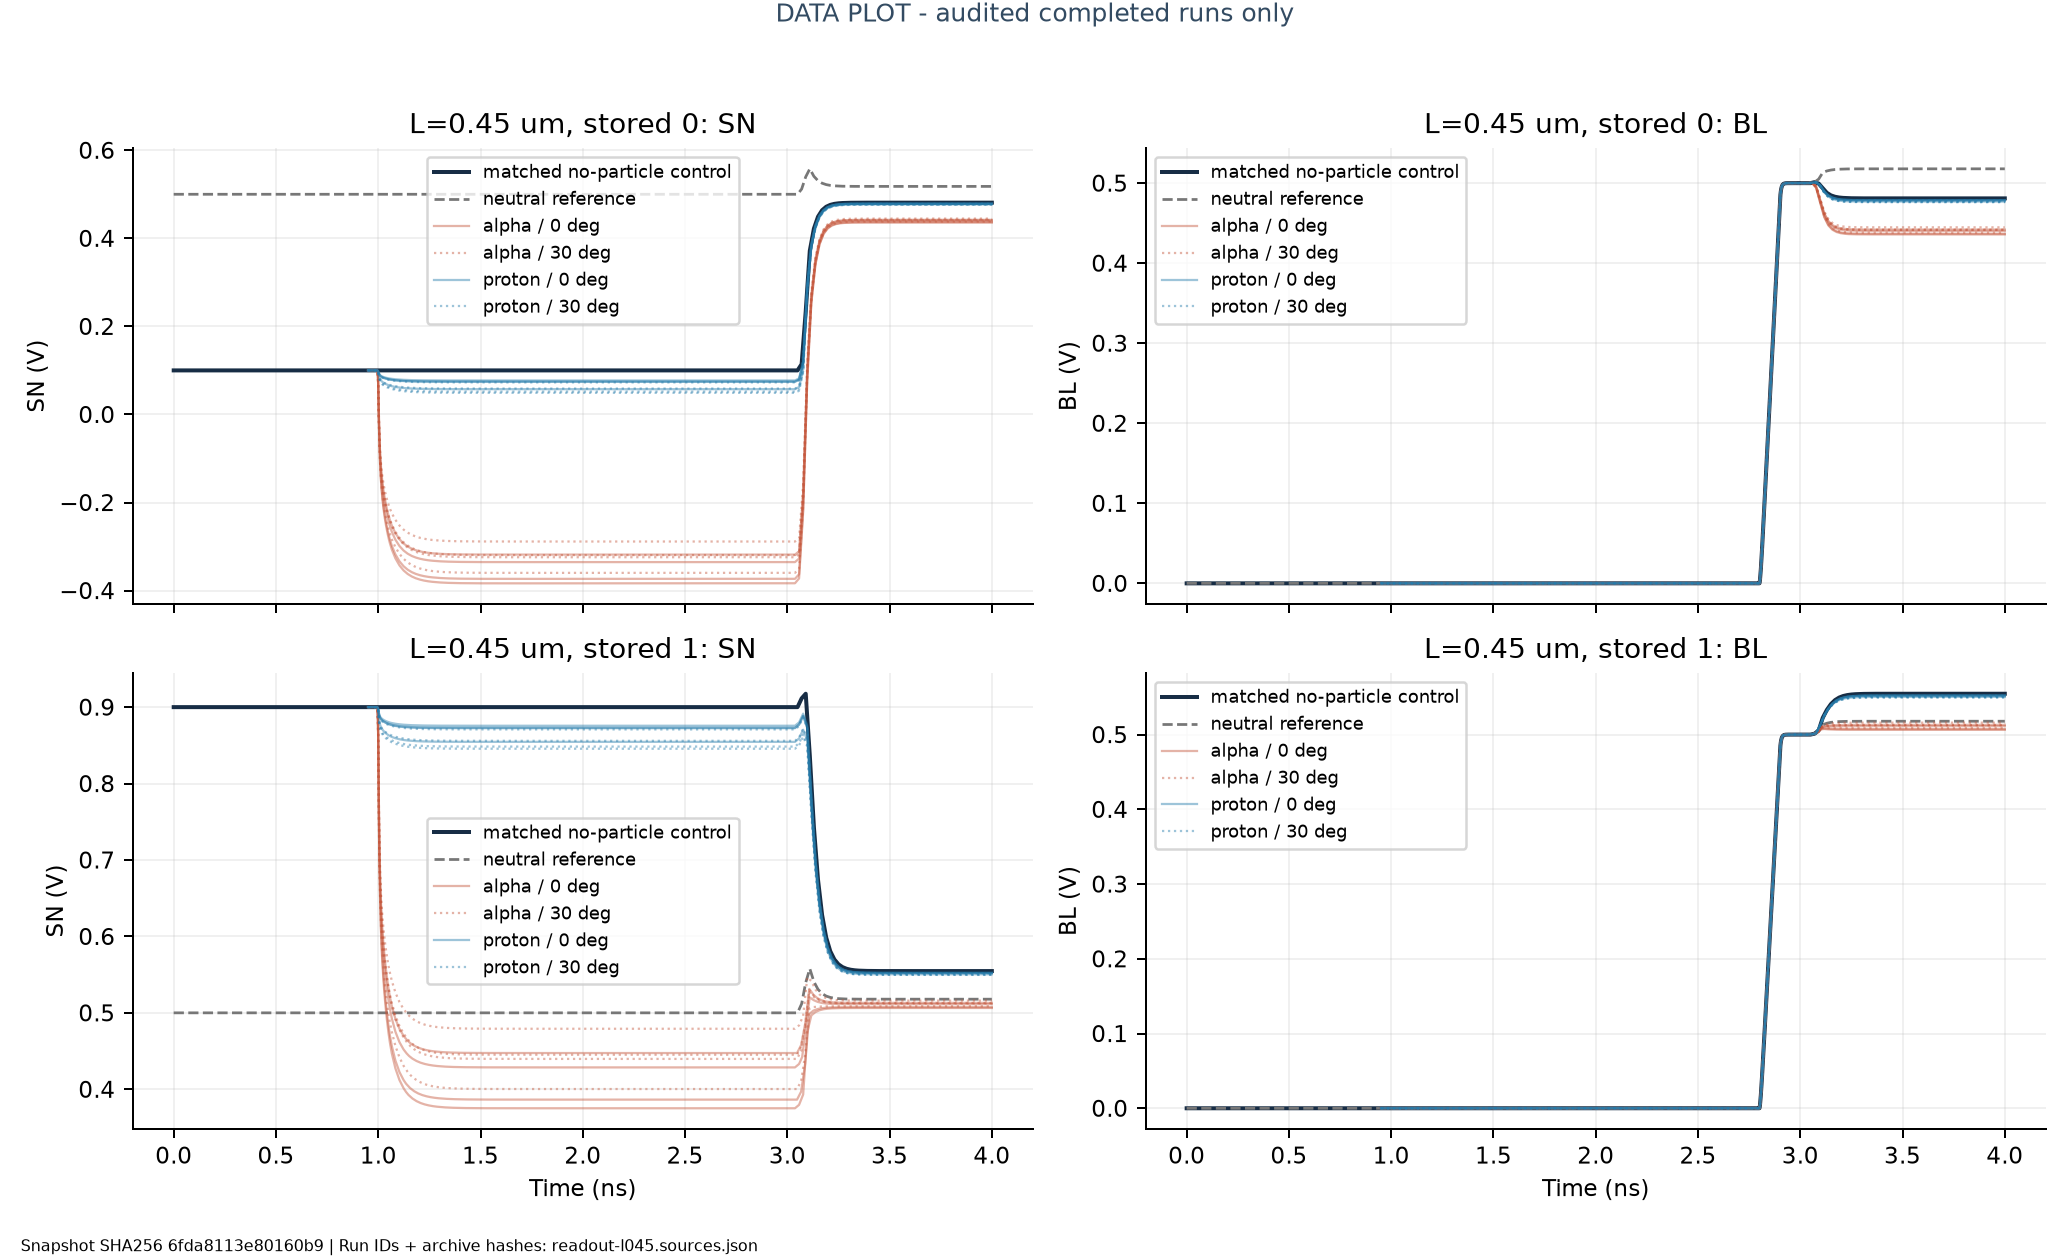
\includegraphics[width=0.48\textwidth]{figures/readout-l045.png}
\caption{v3冻结设计下 0.35/0.45\um 读出响应波形。数据版本：20261012T0033Z-full；误读不等于持久翻转。}
\label{fig:readout-l045}
\end{figure}

\subsection{分类统计与不确定性}

5\mV 主阈值下 128 条配对响应分类为 96 正确、20 判据误读、8 临界、4 数值不确定（图\ref{fig:stratum-counts}）；临界与数值不确定不并入正确，也不改写为已证翻转。图\ref{fig:stratum-intervals} 给出分层统计区间：每物理条件每 bit 的计划独立事件 $N=4$，不是截面，也不是同时覆盖所有分层的 95\% 区间。

\begin{figure}[htbp]
\centering
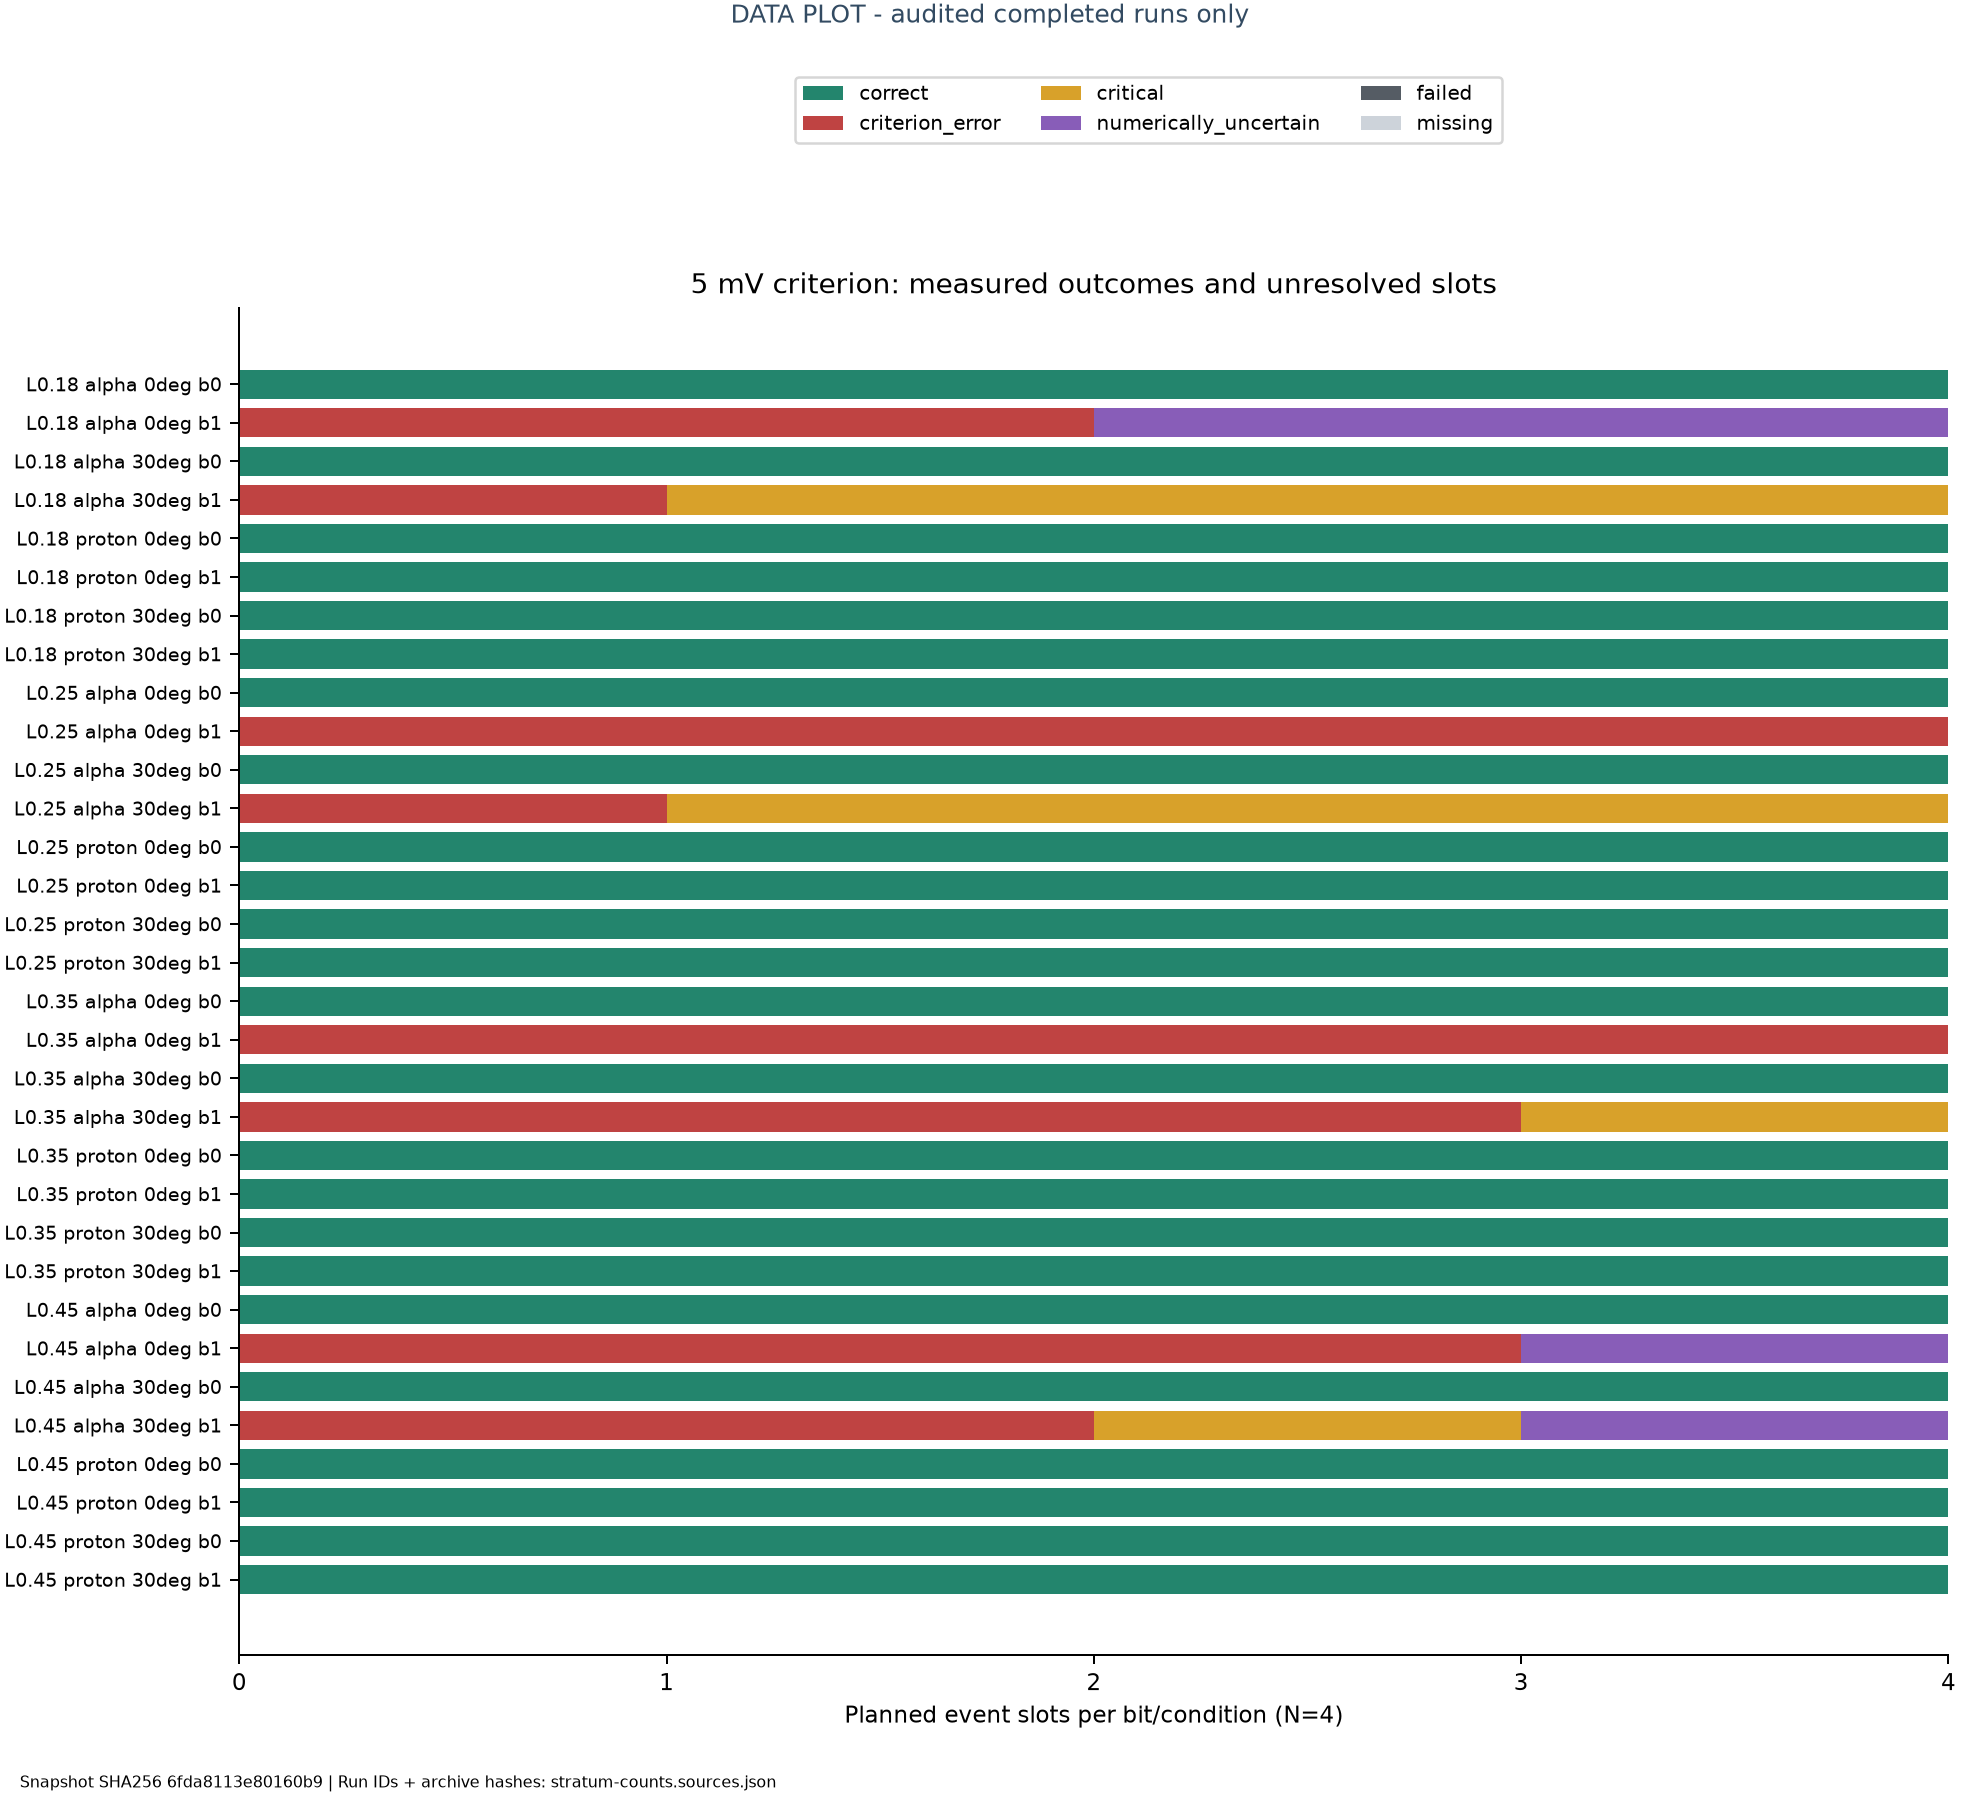
\includegraphics[width=0.7\textwidth]{figures/stratum-counts.png}
\caption{v3冻结设计下主阈值分类计数（正确/误读/临界/数值不确定），共 64 独立事件/128 配对响应，不删除未决。数据版本：20261012T0033Z-full。}
\label{fig:stratum-counts}
\end{figure}
\begin{figure}[htbp]
\centering
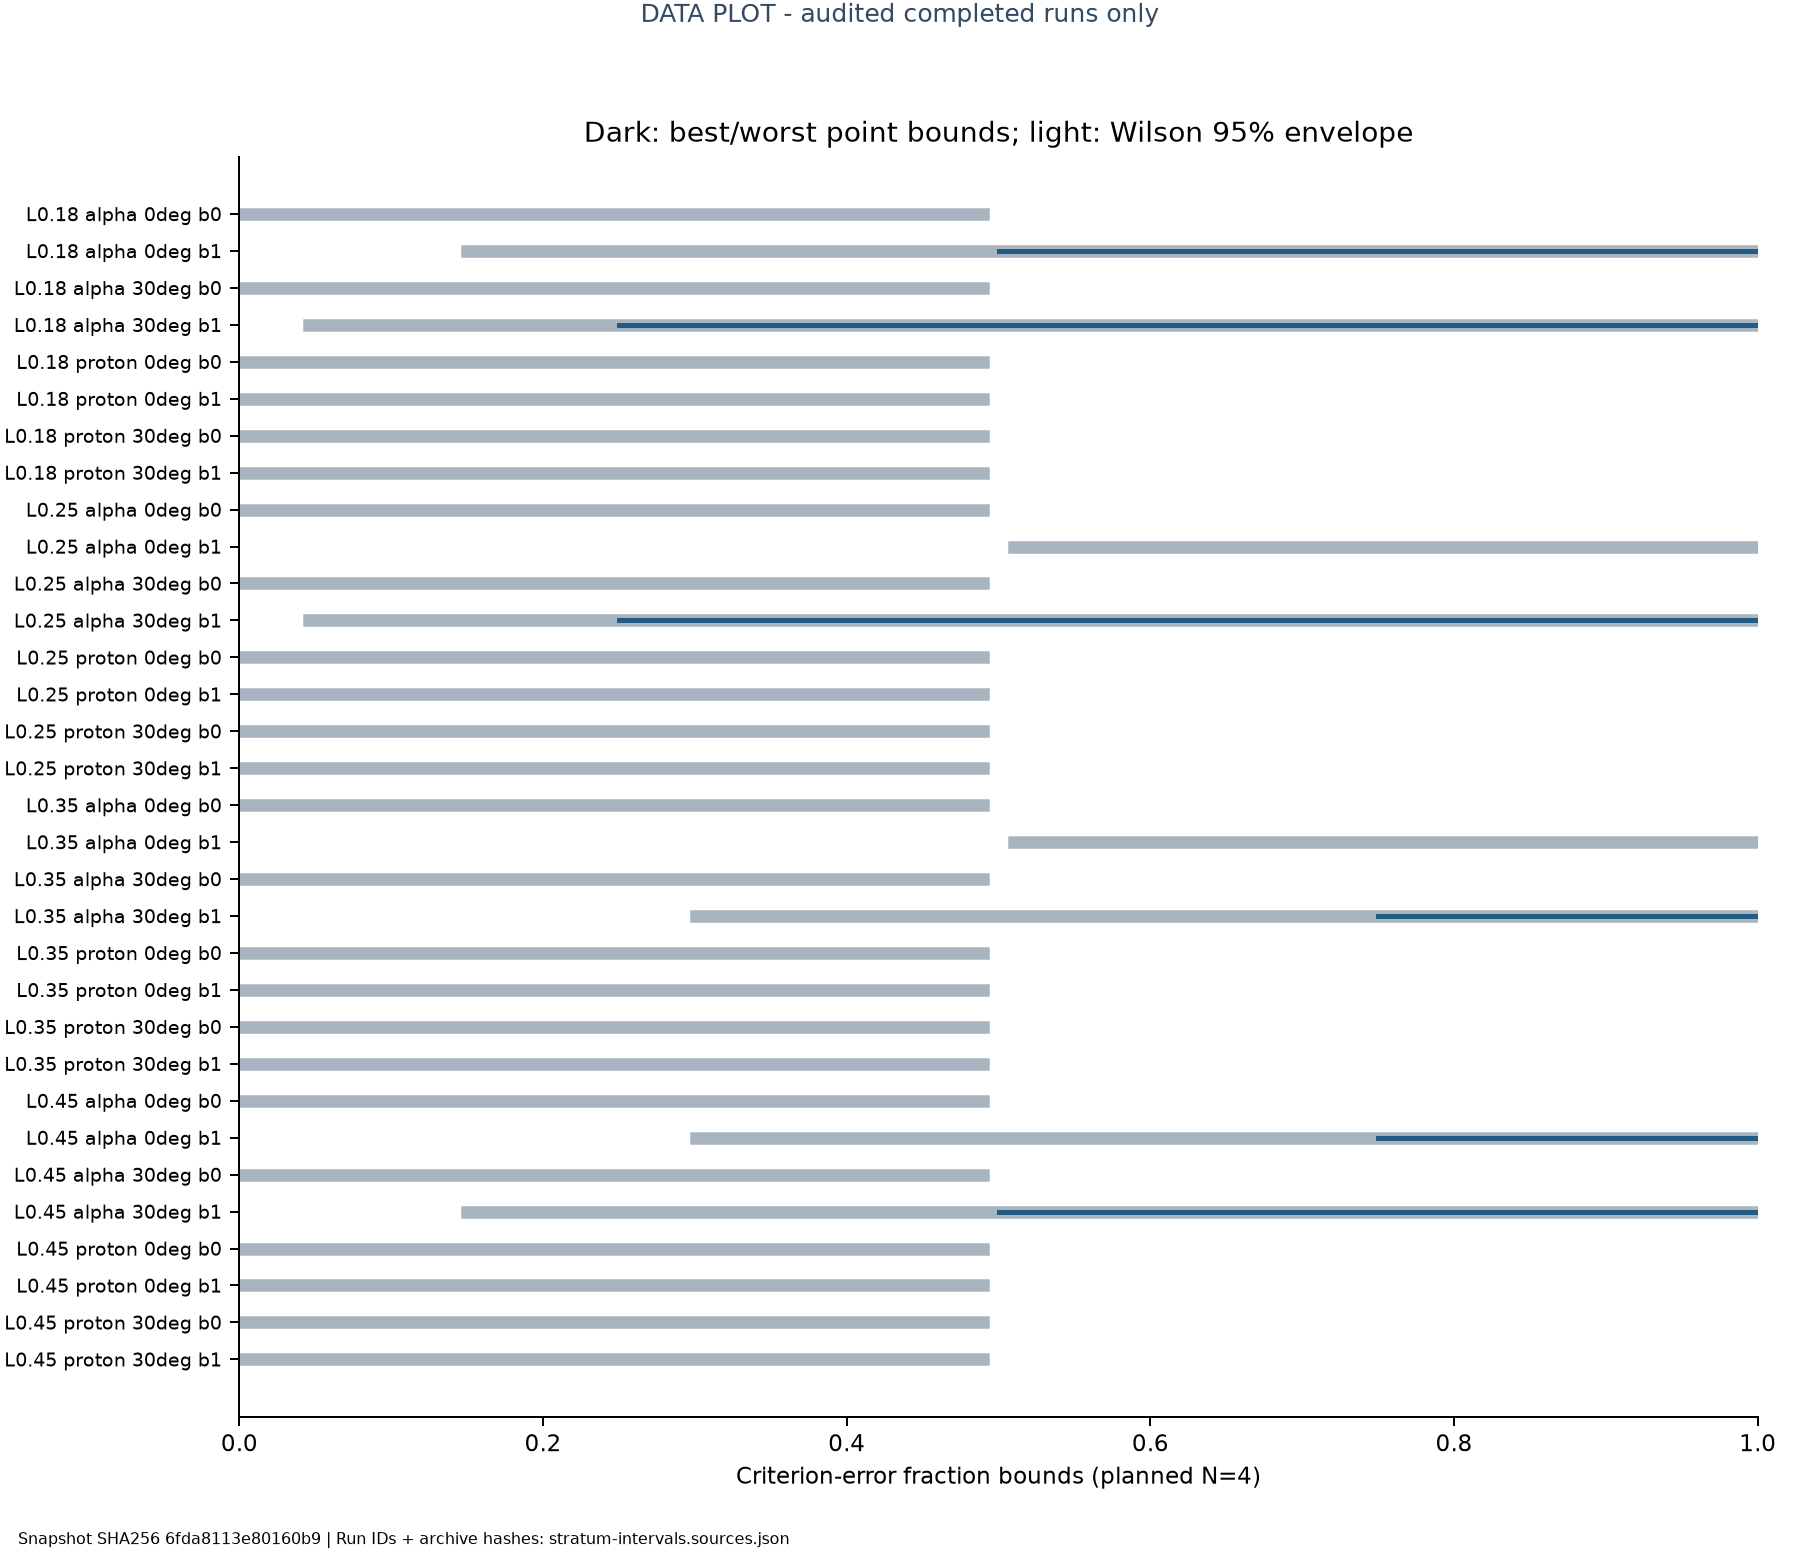
\includegraphics[width=0.7\textwidth]{figures/stratum-intervals.png}
\caption{v3冻结设计下分层统计区间（小样本与未决带来的不确定性）；每条件每 bit $N=4$，不是截面。数据版本：20261012T0033Z-full。}
\label{fig:stratum-intervals}
\end{figure}

\subsection{阈值与读窗敏感性}

图\ref{fig:threshold-l018}--\ref{fig:threshold-l045} 展示 2.5/5/10\mV 阈值与 3.8--4\ns 读窗敏感性；4\ns 单点分类与整个读窗稳定性分开报告。

\begin{figure}[htbp]
\centering
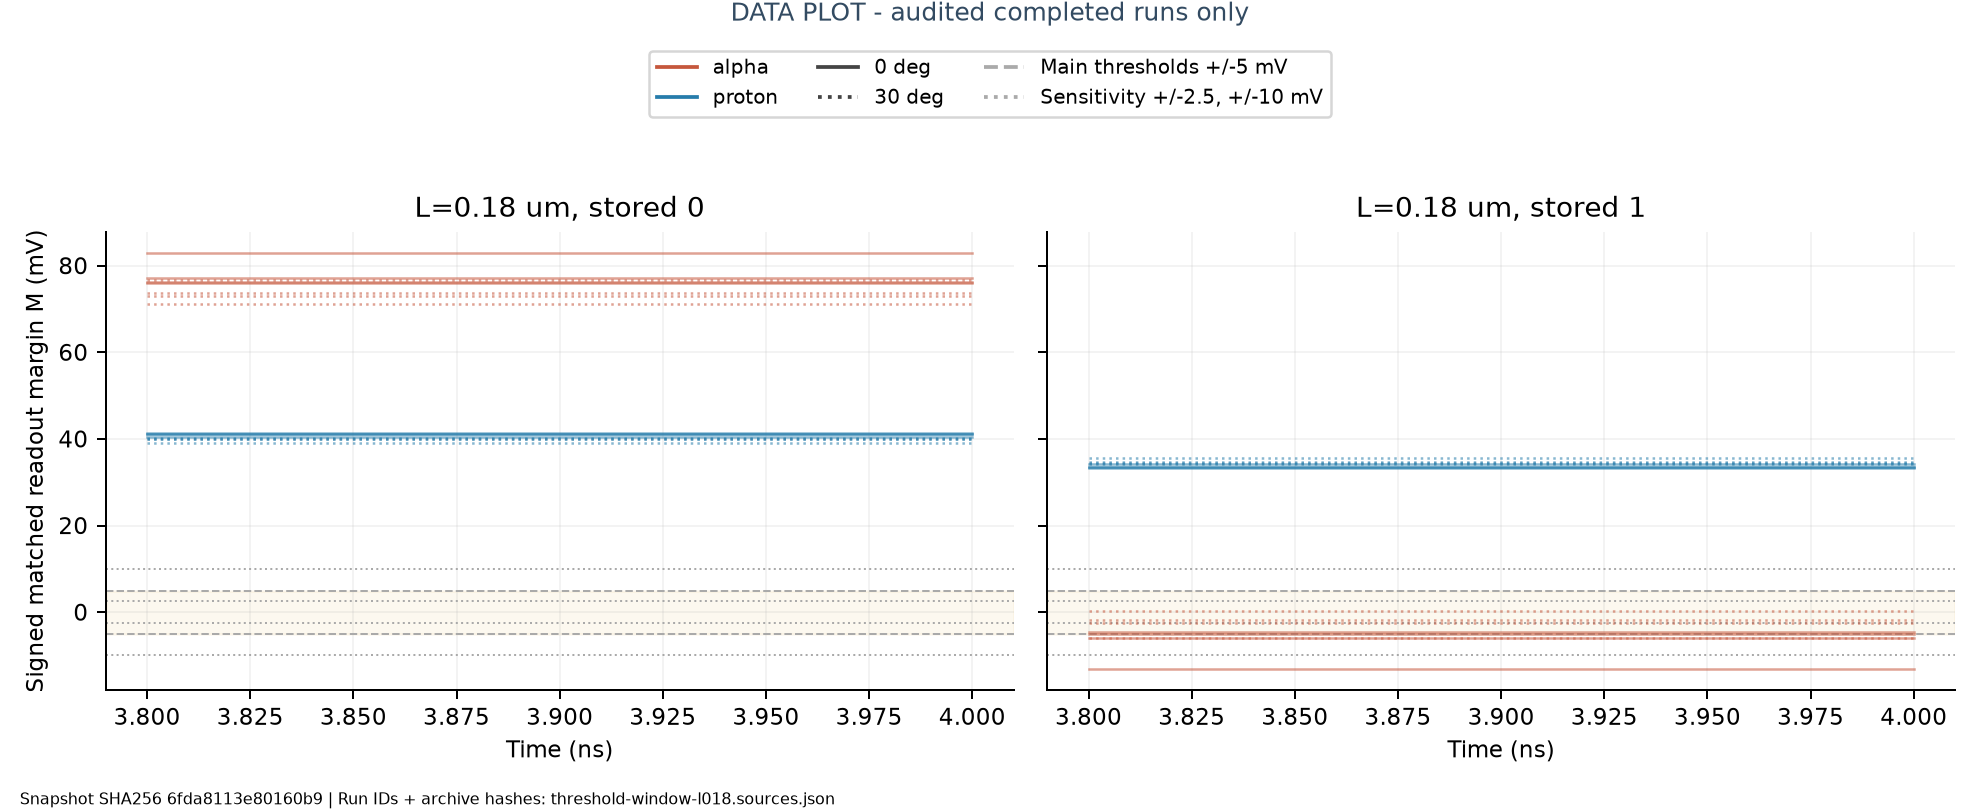
\includegraphics[width=0.48\textwidth]{figures/threshold-window-l018.png}
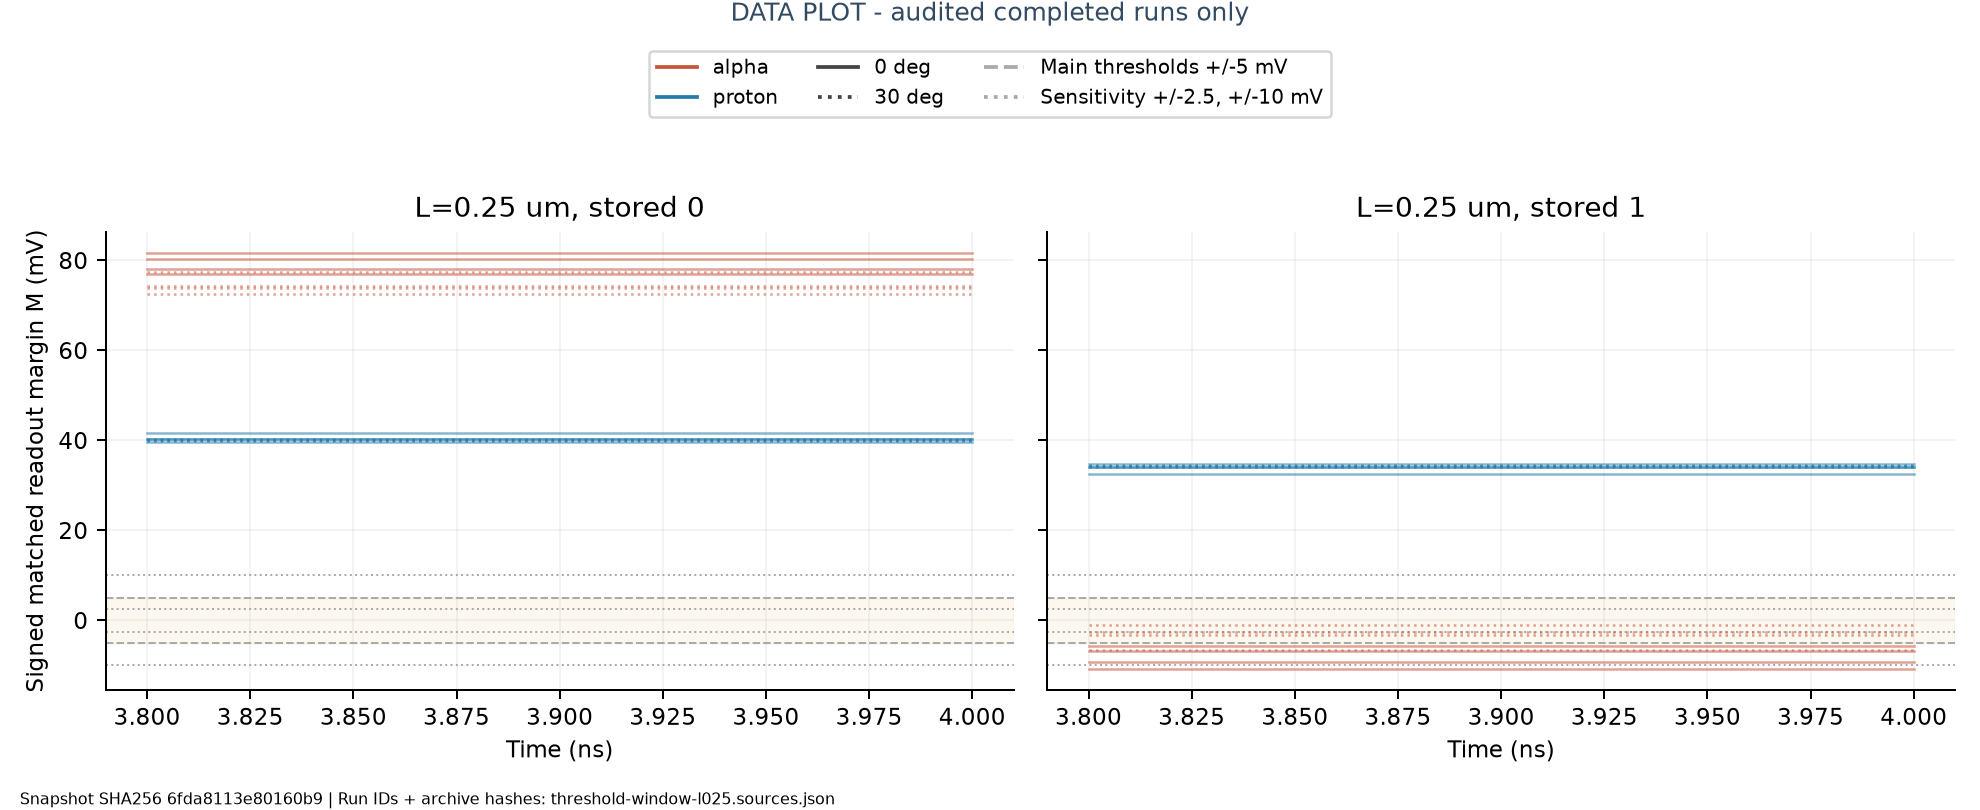
\includegraphics[width=0.48\textwidth]{figures/threshold-window-l025.png}
\caption{v3冻结设计下 0.18/0.25\um 的阈值与读窗敏感性。数据版本：20261012T0033Z-full；v4 阈值须另按基准冻结。}
\label{fig:threshold-l018}
\end{figure}
\begin{figure}[htbp]
\centering
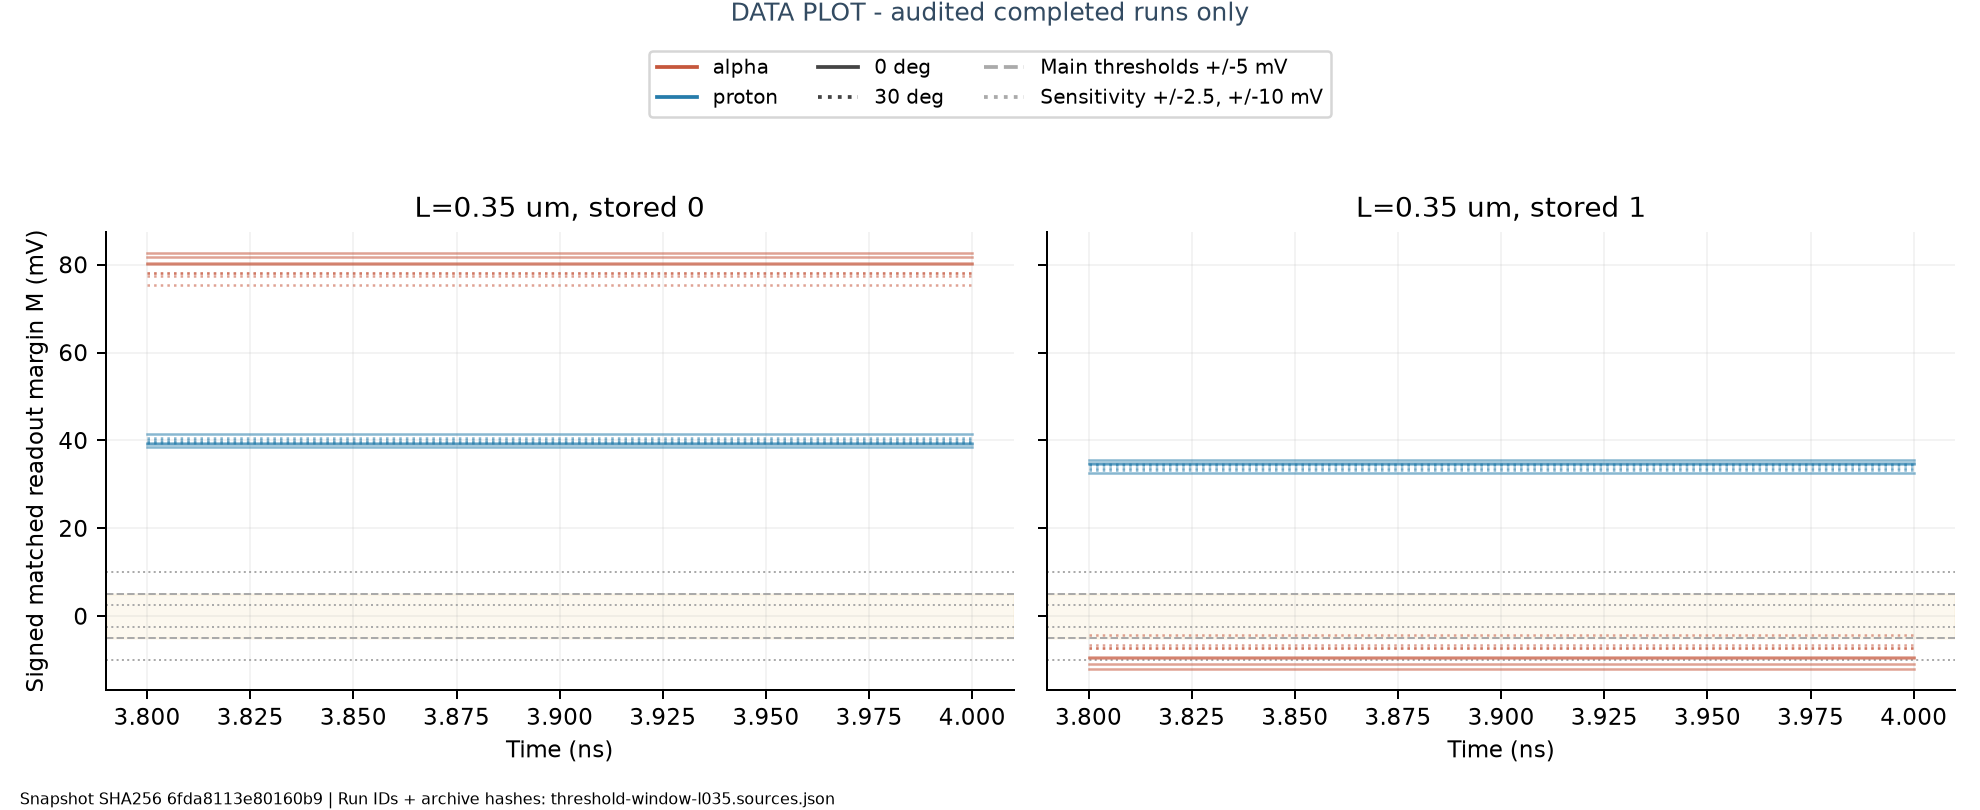
\includegraphics[width=0.48\textwidth]{figures/threshold-window-l035.png}
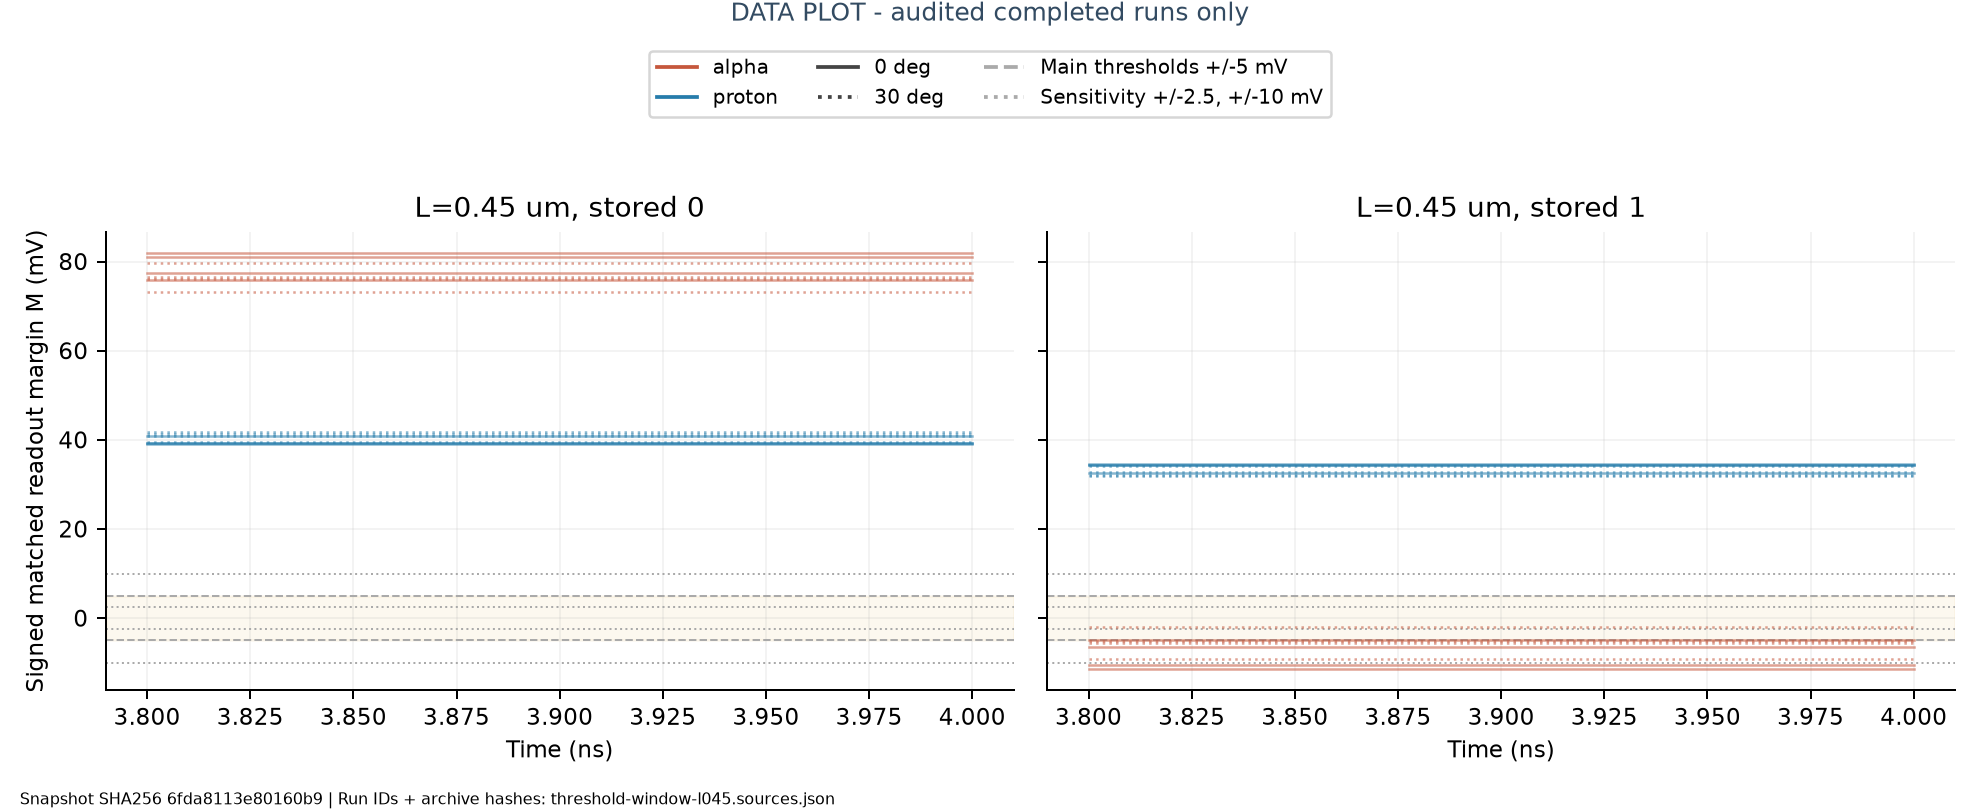
\includegraphics[width=0.48\textwidth]{figures/threshold-window-l045.png}
\caption{v3冻结设计下 0.35/0.45\um 的阈值与读窗敏感性。数据版本：20261012T0033Z-full。}
\label{fig:threshold-l045}
\end{figure}

\subsection{氧化层厚度局部敏感性}

图\ref{fig:oxide} 为固定事件 4/5/6\,nm 氧化层对照：最大变化约 0.11256\mV / 0.00578\fC，小于原容差，不宣称显著工艺效应；属于固定事件局部分析，不扩展为统计规律。

\begin{figure}[htbp]
\centering
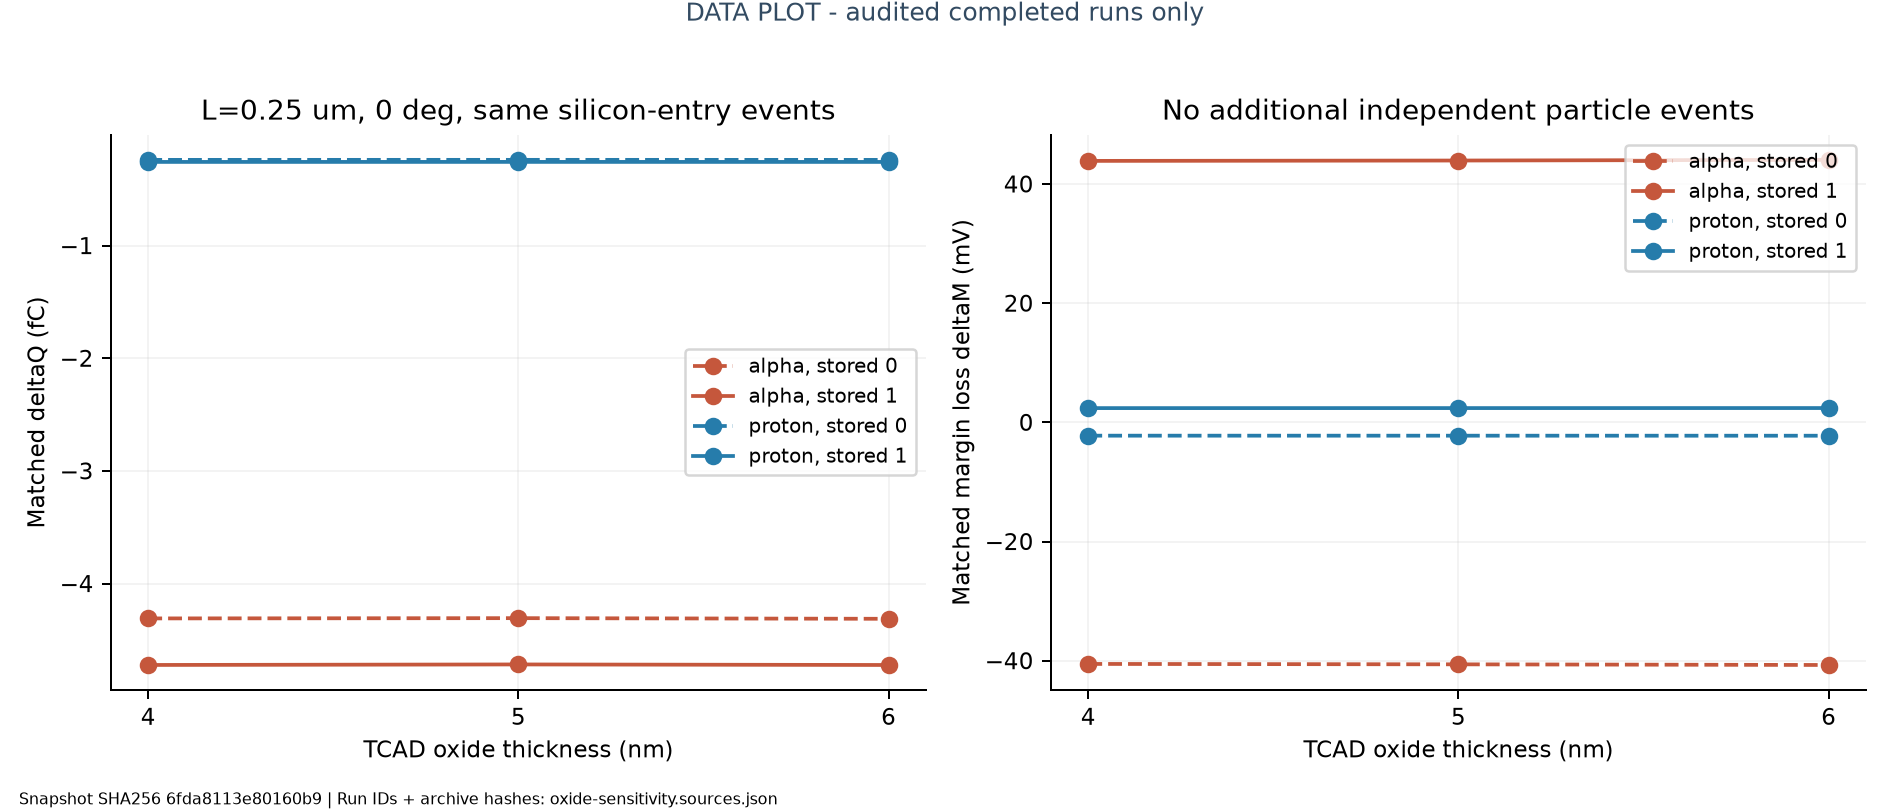
\includegraphics[width=0.7\textwidth]{figures/oxide-sensitivity.png}
\caption{v3冻结设计下 4/5/6\,nm 氧化层固定事件局部敏感性；最大变化约 0.11256\mV/0.00578\fC，小于容差。数据版本：20261012T0033Z-full。}
\label{fig:oxide}
\end{figure}

\subsection{历史预测基线：域内/域外误差}

图\ref{fig:residuals} 与表\ref{tab:pred-dm}--\ref{tab:pred-dq} 给出四个岭回归模型在原冻结划分下的预测残差与误差（域内 $\Delta M$ MAE 约 0.53--0.55\mV）。旧冻结划分；$Q_{dep}$ 等特征依赖 Geant4，推理成本不能省略输运；该基线不冒充新模型的独立盲测。

\begin{figure}[htbp]
\centering
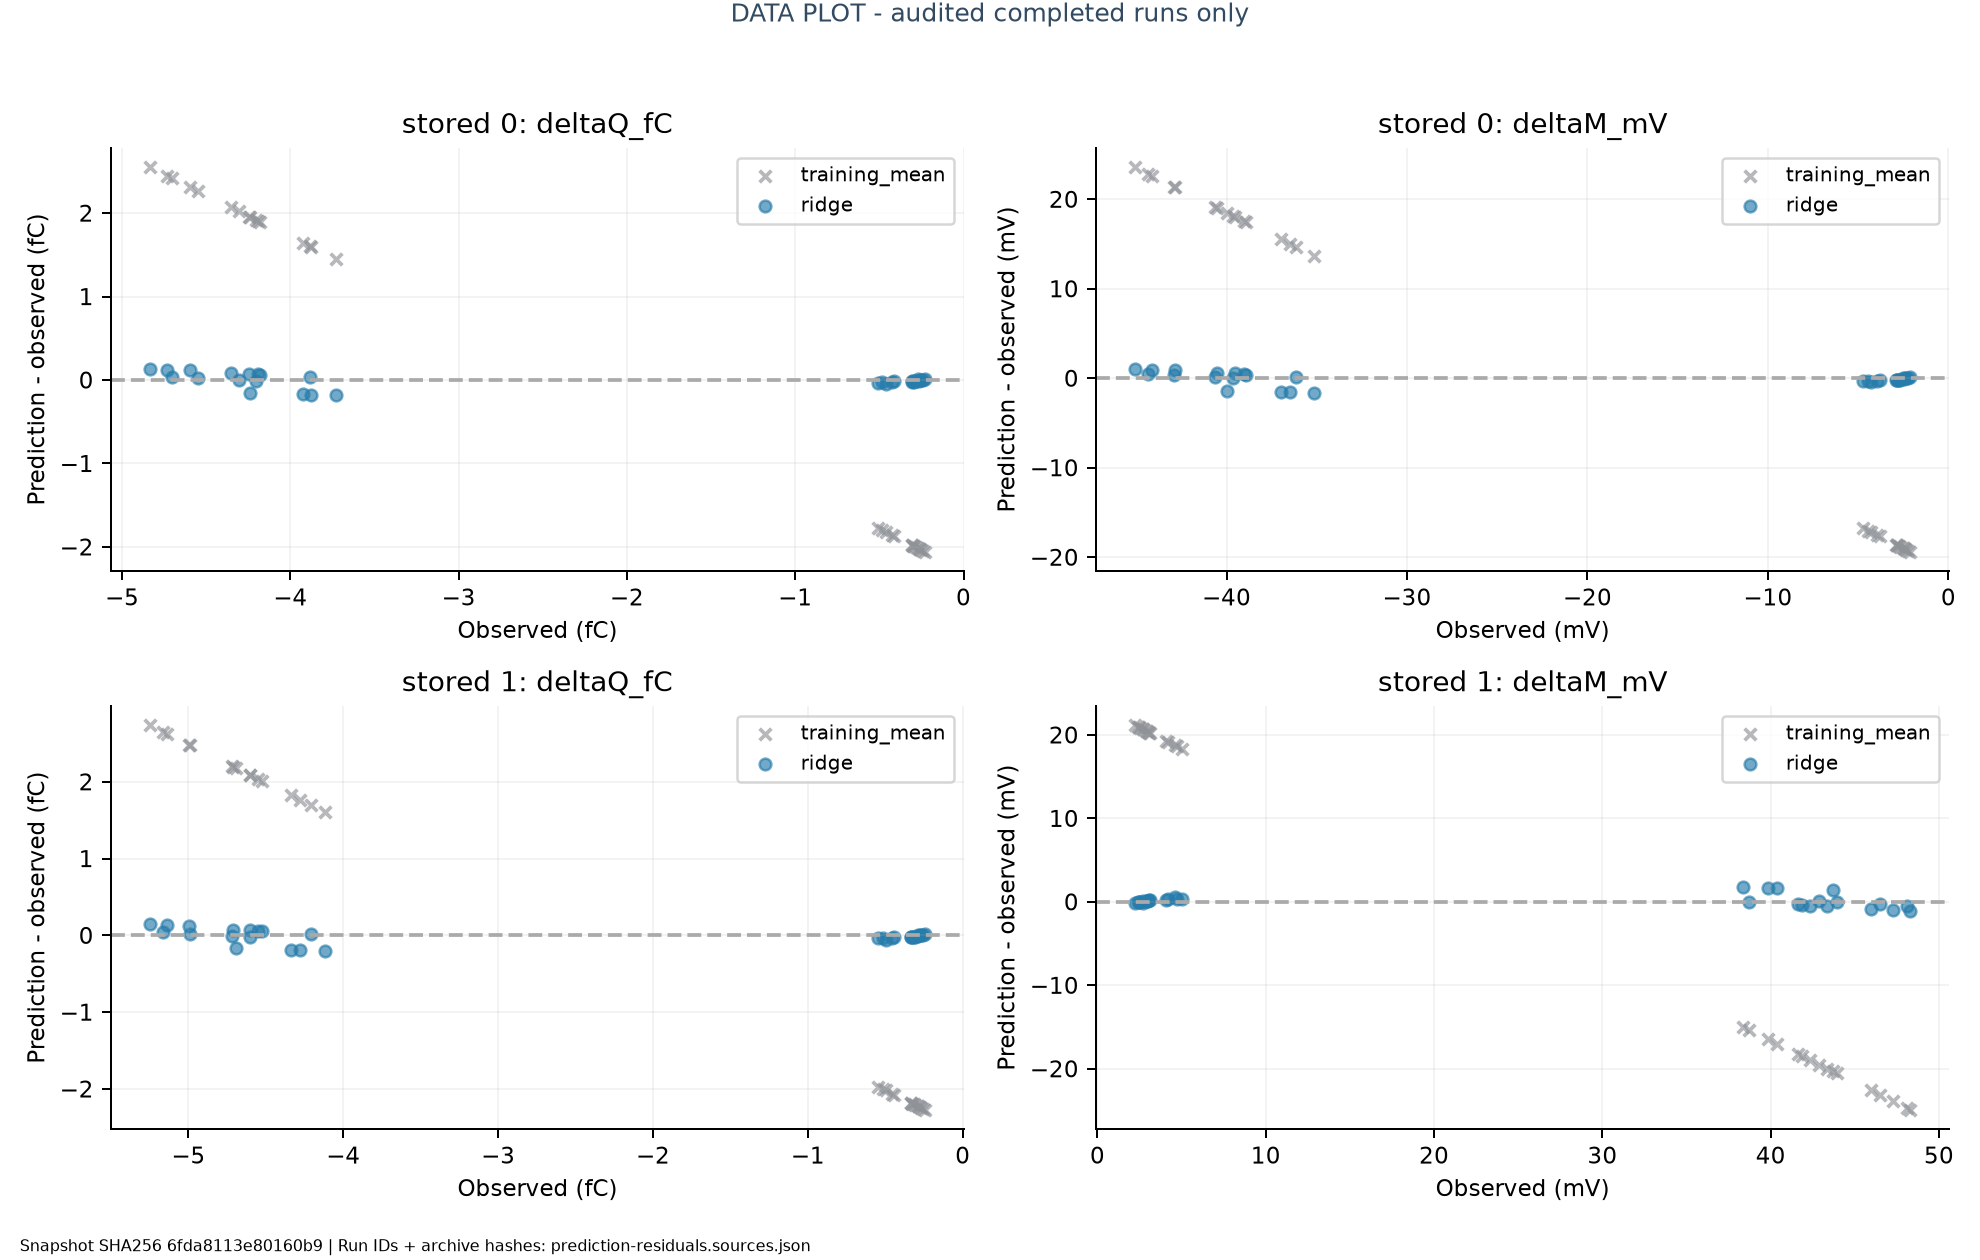
\includegraphics[width=0.75\textwidth]{figures/prediction-residuals.png}
\caption{v3冻结设计下岭回归与均值基线的预测残差（域内/域外、两目标）；旧冻结划分，特征含 Geant4 沉积。数据版本：20261012T0033Z-full。}
\label{fig:residuals}
\end{figure}
\begin{table}[htbp]
\centering\small
\caption{裕量预测误差（mV），按 bit、域内/域外与模型分开}
\label{tab:pred-dm}
\begin{tabular}{lllrrrrrr}
\toprule
集合 & 位 & 模型 & $n$ & 缺失 & 无效 & MAE & RMSE & 最大误差\\
\midrule
留出 & 0 & 均值基准 & 16 & 0 & 0 & 18.320612 & 18.448022 & 22.860163\\
留出 & 0 & 岭回归 & 16 & 0 & 0 & 0.526964 & 0.798415 & 1.645649\\
留出 & 1 & 均值基准 & 16 & 0 & 0 & 19.936695 & 20.066626 & 24.741705\\
留出 & 1 & 岭回归 & 16 & 0 & 0 & 0.549768 & 0.838043 & 1.765441\\
外推 & 0 & 均值基准 & 16 & 0 & 0 & 18.742144 & 18.867683 & 23.569637\\
外推 & 0 & 岭回归 & 16 & 0 & 0 & 0.404964 & 0.519434 & 1.075289\\
外推 & 1 & 均值基准 & 16 & 0 & 0 & 20.091257 & 20.219896 & 24.915029\\
外推 & 1 & 岭回归 & 16 & 0 & 0 & 0.387723 & 0.504929 & 1.105078\\
\bottomrule
\end{tabular}

\end{table}
\begin{table}[htbp]
\centering\small
\caption{电荷预测误差（fC），不与 mV 混合平均}
\label{tab:pred-dq}
\begin{tabular}{lllrrrrrr}
\toprule
集合 & 位 & 模型 & $n$ & 缺失 & 无效 & MAE & RMSE & 最大误差\\
\midrule
留出 & 0 & 均值基准 & 16 & 0 & 0 & 1.942616 & 1.956036 & 2.416036\\
留出 & 0 & 岭回归 & 16 & 0 & 0 & 0.056607 & 0.088294 & 0.181592\\
留出 & 1 & 均值基准 & 16 & 0 & 0 & 2.140865 & 2.154850 & 2.651122\\
留出 & 1 & 岭回归 & 16 & 0 & 0 & 0.061766 & 0.094644 & 0.198945\\
外推 & 0 & 均值基准 & 16 & 0 & 0 & 2.011262 & 2.025386 & 2.548969\\
外推 & 0 & 岭回归 & 16 & 0 & 0 & 0.052826 & 0.068049 & 0.136393\\
外推 & 1 & 均值基准 & 16 & 0 & 0 & 2.183932 & 2.198297 & 2.733561\\
外推 & 1 & 岭回归 & 16 & 0 & 0 & 0.051740 & 0.067155 & 0.144228\\
\bottomrule
\end{tabular}

\end{table}

\subsection{原生软件窗口证据}

图\ref{fig:native-phys}（左、右两幅）为完整原生窗口（非裁切）：保留图例、单位与坐标轴定义（Abs(ElectricField-V)，V/cm；SVisual 竖向 X/横向 Y）。F01--F13 为真实数据生成的 DATA PLOT，本两图才是原生窗口证据。

\begin{figure}[htbp]
\centering
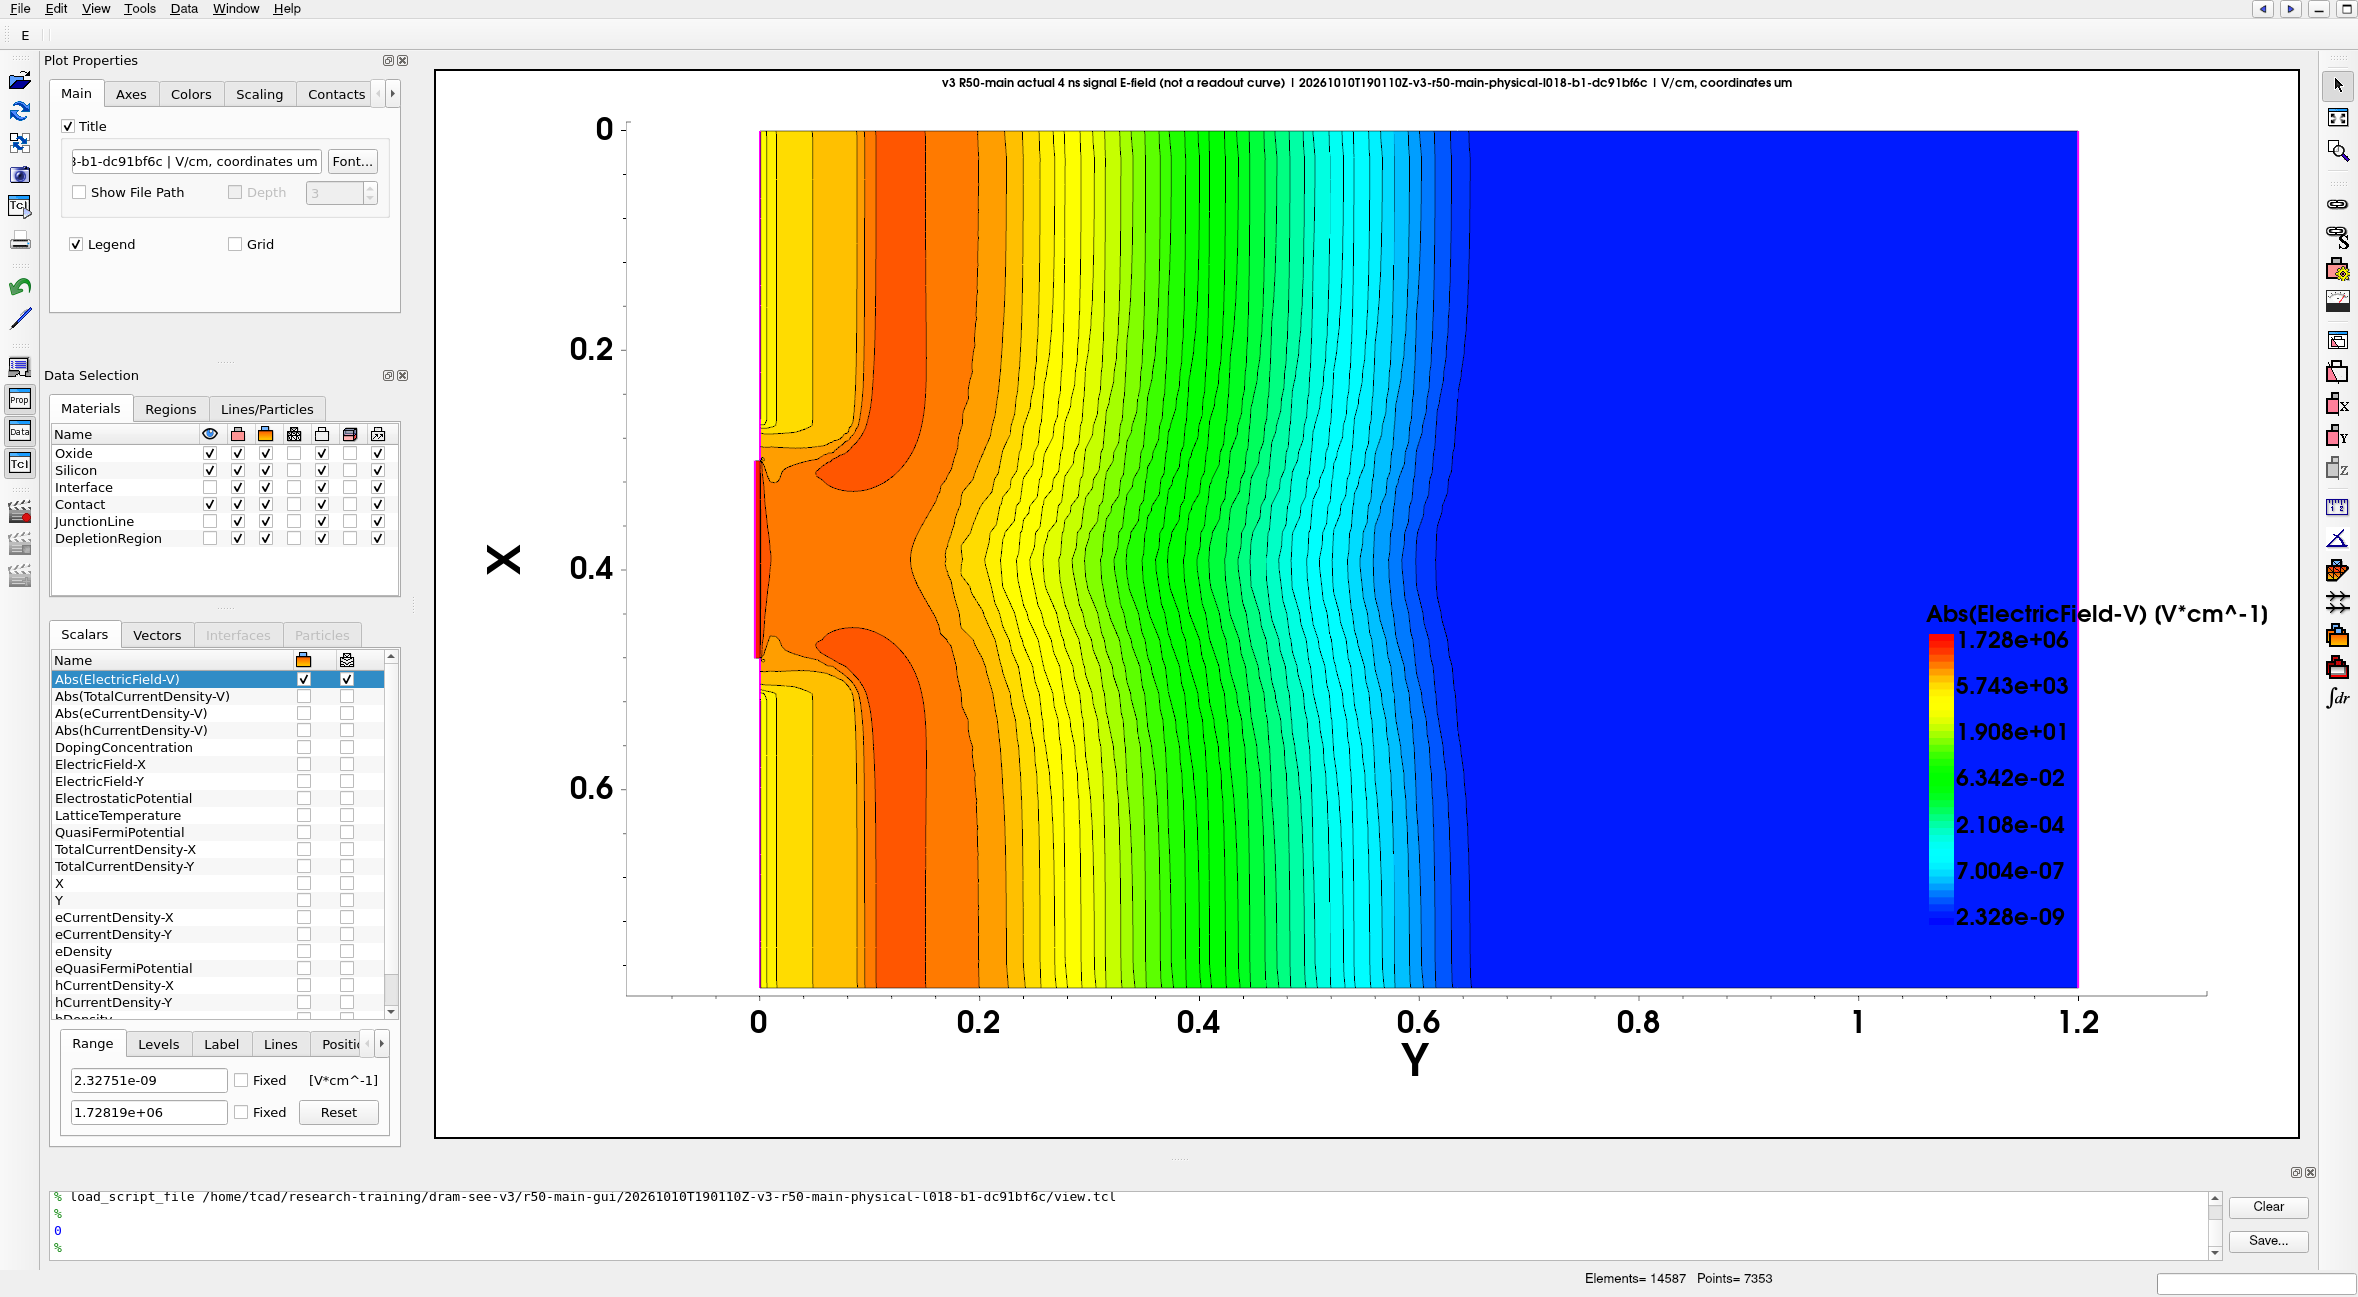
\includegraphics[width=0.48\textwidth]{figures/native-physical-window.png}
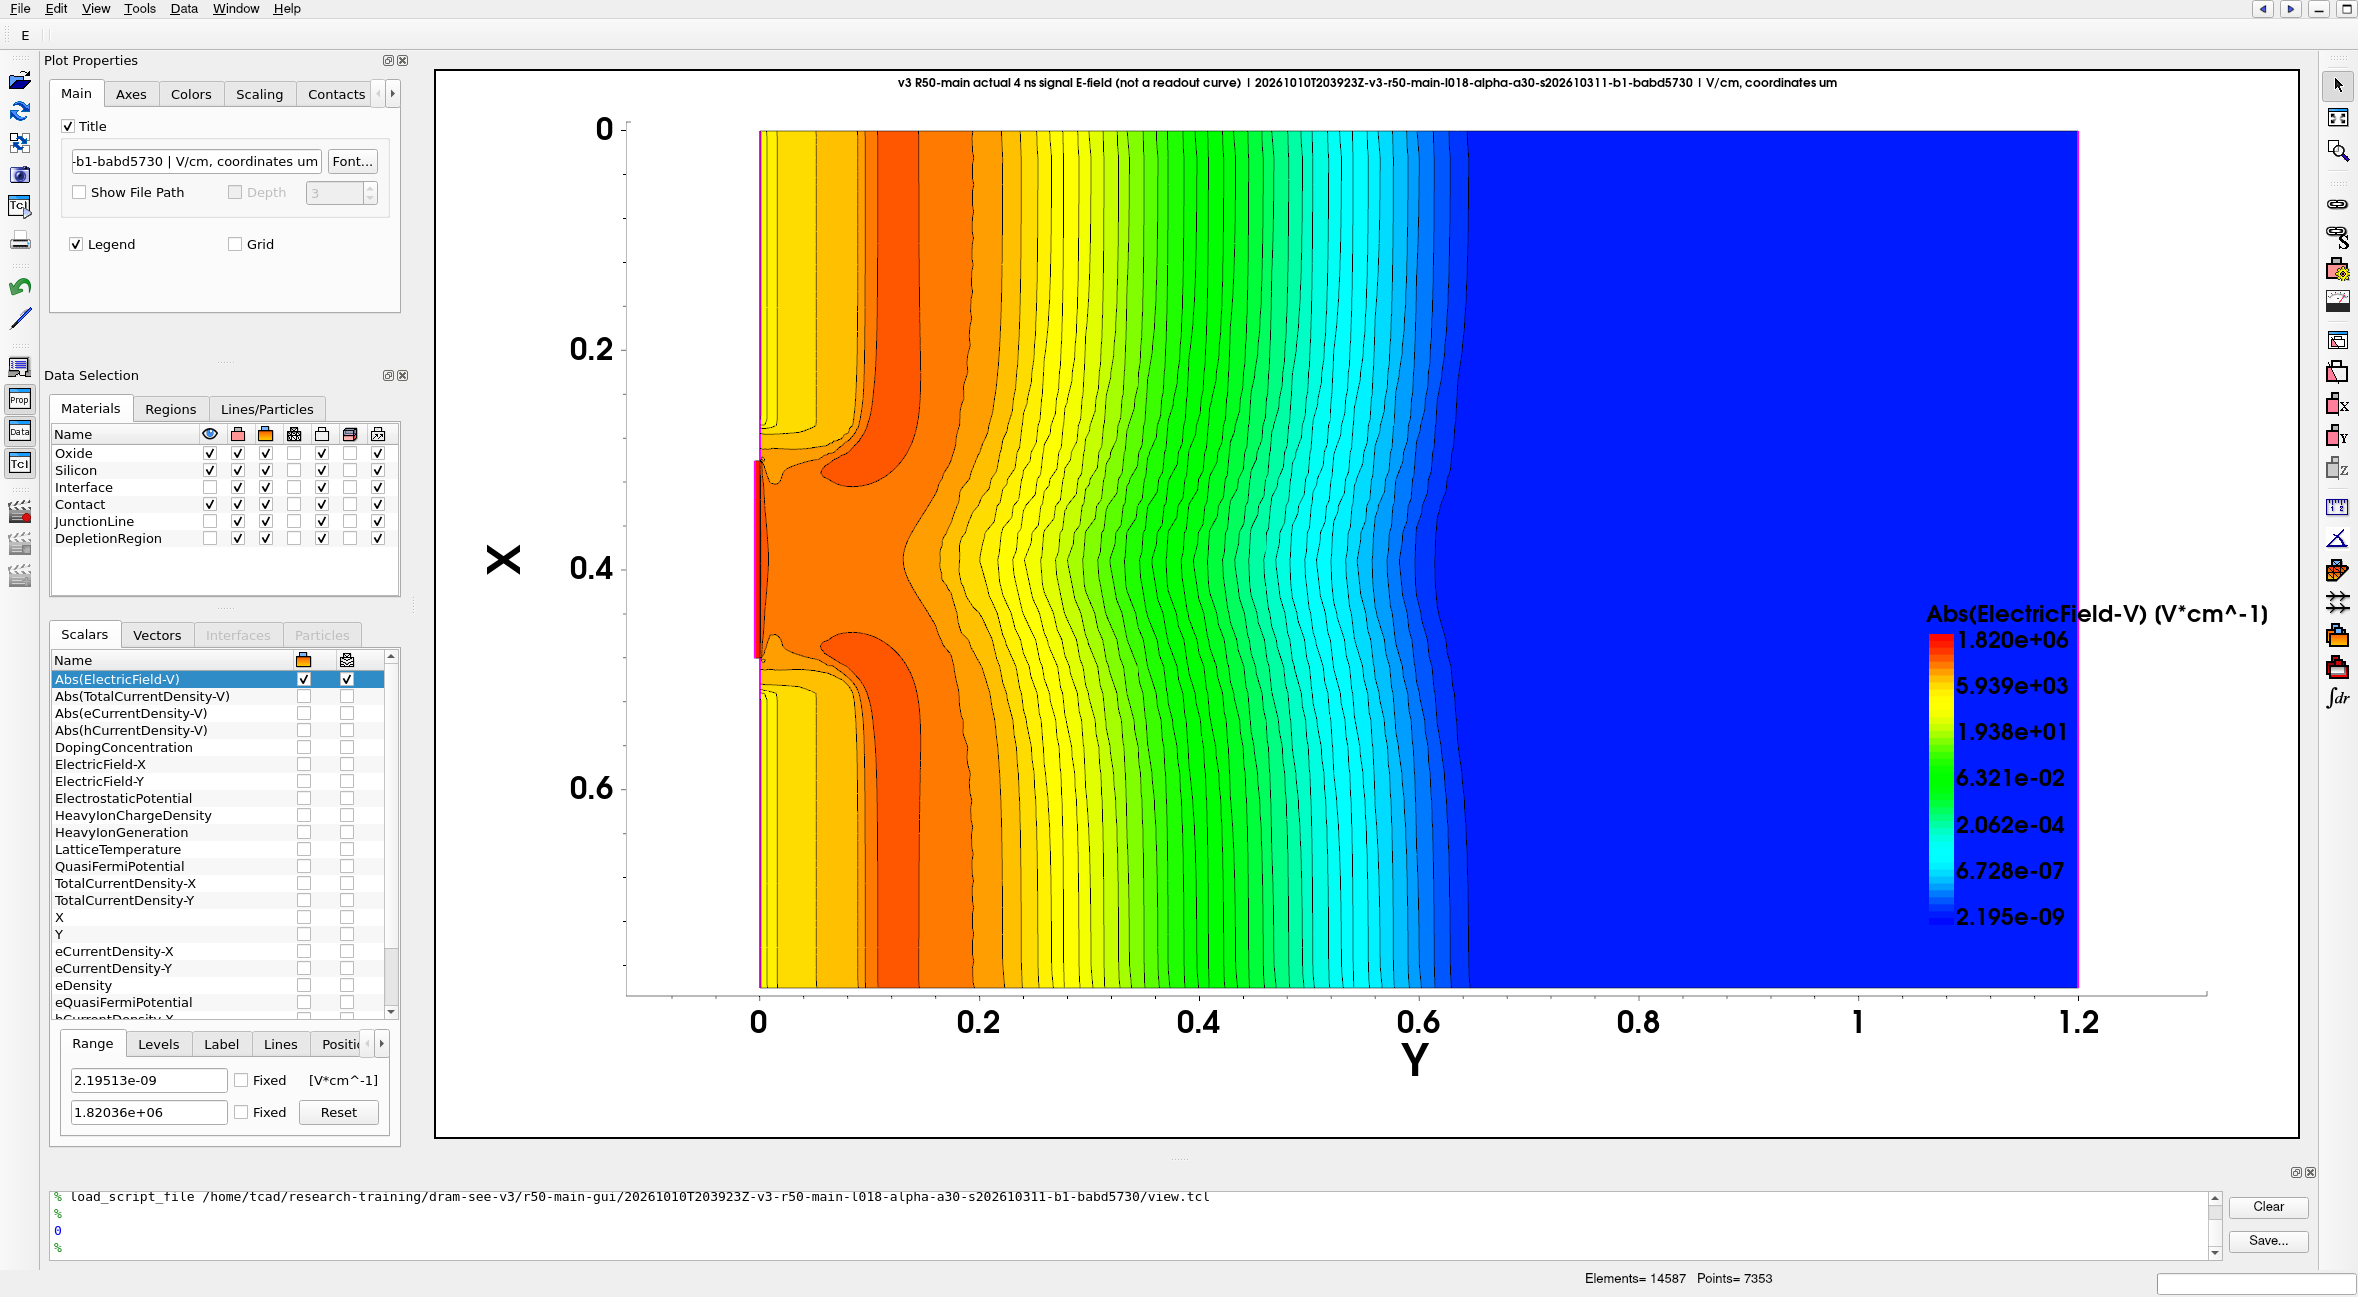
\includegraphics[width=0.48\textwidth]{figures/native-event-window.png}
\caption{v3原生模型/场分布窗口（左）与指定事件 4\ns 电场分布（右）；Abs(ElectricField-V)，V/cm，勿擅自换轴。数据版本：20261012T0033Z-full。}
\label{fig:native-phys}
\end{figure}

\subsection{待补：r0.6 新结果与成本统计}

\textbf{待补。} D0--D3 第一波合格结果、吞吐/资源图（单/双/三任务）、v4 两 bit 全周期与 KCL、α/质子源资格图、数据覆盖矩阵、AI 消融与分组 CV、截面/外部对比——先有合格数据再画图，清单见 \texttt{materials/图表引用清单.md} 的"下一批待补图"。

% 第6章 讨论：误差来源、失败案例、适用边界与关键影响因素（占位）
% 素材：experiments/dram-see-v3/blocker.md、diagnostic-report.md（预充失败复盘）；
%       experiments/dram-see-v4/source-field-audit-r1（粗网格空间失败保留）；
%       shared/literature/mentor-added-20261116.md（四类机制区分：瞬态收集/SEFI/位移损伤保持退化/BTI）；
%       缺口：A04 截面/错误率与外部验证（需 G01/G04 分母与导师实验数据 M01/M02）
\section{讨论}

\textbf{待补章节。} 本章计划讨论：数值误差 vs 判据误差 vs 物理机制的分层解释；失败案例（预充门槛、粗网格空间失败）的原因与边界；模型泛化到未见工况的能力；关键影响因素（尺寸、粒子、角度、温度等）的物理解释；与导师实验数据的对比（待交接）。

% 第7章 结论与展望
% 红线：只写证据支撑的结论；计划/待补事项明确标"待完成"，不写"显著提高"等无证据表述
% 证据：前六章各节注释；素材总览见 materials/素材索引.md
\section{结论与展望}

\subsection{主要结论}

本文围绕《AI辅助下的DRAM存储器单粒子效应评估研究》，建立了从 Geant4 粒子输运到 TCAD 器件响应的可审计联合建模与数据链路，统一了指标与标签口径，构建了带 run ID 与哈希的冻结数据集，并设计了 R$\rightarrow$A$\rightarrow$F 数据驱动预测链路与物理约束消融、分组交叉验证、冻结盲测协议。已有证据支持以下结论：

\begin{enumerate}
  \item 在 v3 冻结设计（未校准二维代表模型、固定 5\,MeV、两角度、固定入射位置）下，64 个独立事件 / 128 条配对响应可按匹配对照与 $\varepsilon=5\mV$ 主阈值严格分类（96 正确 / 20 判据误读 / 8 临界 / 4 数值不确定），预登记数值细化在容差内、失败案例（3\ns 预充偏差 13.297\uV）被保留而非掩盖——方法链路的可复现性得到验证。
  \item 基于沉积电荷、栅长与角度特征的岭回归基线在八工况留一交叉验证中显著优于均值基准（$\Delta Q$ 折 RMSE 0.103/0.113\fC，$\Delta M$ 0.955/1.012\mV），域内 $\Delta M$ MAE 约 0.53--0.55\mV，支持"给定源项与基线条件下，低维回归可作 TCAD 响应代理"的域内可行性。
  \item v4/r0.6 阶段在厚硅输运与三维源接口上取得阶段性资格证据（212 初级事件、9 条核非弹性记录、三个三维源账本闭合、细网格 A0/A1 全帧通过），P0 四项资格门与 D0--D3 第一波正在推进。
\end{enumerate}

\subsection{局限与待补}

本文的器件结论限于未校准代表模型，不代表真实 DDR5；判据误读不等于持久位翻转；配对响应与复跑不增加独立样本。以下事项\textbf{待完成}，不在本稿中宣称：v3 插值/外推留出的全量独立验收与新模型的冻结盲测；r0.6 合格数据集导出与 R/A/F 正式训练；物理约束消融的定量比较；带注量/分母的截面与错误率；与导师课题组 DDR5 实验原始数据（M01/M02）的外部对比；真实器件 I--V/保持/读出校准（M04/M05）。

\subsection{后续工作}

后续按 r0.6 排批推进 P0 资格门与 D0--D3/LHS 合格数据，导出可训练快照后启动 R/A/F 训练与消融、分组 CV 及冻结盲测；同步推进向导师交接实验原始数据、器件校准依据与毕业设计模板（M01/M02/M04/M06），补齐统计分母后开展截面/错误率与外部验证，并按学校模板完成三门课成稿。


\FloatBarrier
\bibliographystyle{unsrt}
\bibliography{refs/references}

\end{document}
